%==============================================================================
%  Weather Forecasting — University Project Report
%  Compile: pdflatex -> bibtex -> pdflatex -> pdflatex  (Overleaf does this auto)
%  Self-contained: the bibliography database is embedded via filecontents below.
%==============================================================================
\documentclass[12pt,a4paper,oneside]{report}  
%------------------------------------------------------------------ Encoding/lang
\usepackage[utf8]{inputenc}
\usepackage[T5]{fontenc}  
\usepackage[T1]{fontenc}
\usepackage{textcomp}
\usepackage[english]{babel}
\usepackage{lmodern}

%------------------------------------------------------------------ Layout
\usepackage[a4paper,margin=2.5cm]{geometry}
\usepackage{setspace}
\onehalfspacing
\usepackage{fancyhdr}
\usepackage{emptypage}
\usepackage[titletoc]{appendix}

%------------------------------------------------------------------ Math
\usepackage{amsmath,amssymb,amsfonts,amsthm}
\usepackage{bm}
\usepackage{siunitx}

%------------------------------------------------------------------ Graphics/tables
\usepackage{graphicx}
\graphicspath{{figs/}{./figs/}}   % EDA + XGBoost figures live in report/figs/
\usepackage{float}
\usepackage{booktabs}
\usepackage{array}
\usepackage{multirow}
\usepackage{longtable}
\usepackage{tabularx}
\usepackage{caption}
\usepackage{subcaption}
\usepackage{xcolor}
\usepackage{tikz}
\usetikzlibrary{shapes.geometric, arrows.meta, positioning, fit, backgrounds}

%------------------------------------------------------------------ Algorithms/code
\usepackage{algorithm}
\usepackage{algpseudocode}  % provides the algorithmic environment (algorithmicx)
\usepackage{listings}

%------------------------------------------------------------------ References/links
\usepackage[numbers,sort&compress]{natbib}
\usepackage[hidelinks]{hyperref}
\usepackage[nottoc]{tocbibind}

%------------------------------------------------------------------ Listings style
\definecolor{codegray}{gray}{0.95}
\definecolor{codegreen}{rgb}{0.0,0.45,0.0}
\definecolor{codeblue}{rgb}{0.10,0.10,0.65}
\lstdefinestyle{py}{
  language=Python,
  backgroundcolor=\color{codegray},
  basicstyle=\ttfamily\small,
  keywordstyle=\color{codeblue}\bfseries,
  commentstyle=\color{codegreen}\itshape,
  stringstyle=\color{red!60!black},
  numbers=left, numberstyle=\tiny\color{gray}, numbersep=8pt,
  breaklines=true, frame=single, captionpos=b, showstringspaces=false,
  tabsize=2,
}

%------------------------------------------------------------------ Header/footer
\pagestyle{fancy}
\fancyhf{}
\renewcommand{\headrulewidth}{0.4pt}
\fancyhead[L]{\nouppercase{\leftmark}}
\fancyhead[R]{\thepage}

%------------------------------------------------------------------ Figure placeholder
% Renders a framed box so the document COMPILES with no external image files.
% Replace with \includegraphics when the real figure is ready (see commented lines).
\newcommand{\figplaceholder}[1]{%
  \begin{center}
  \setlength{\fboxsep}{10pt}%
  \fbox{\begin{minipage}[c][0.26\textheight][c]{0.82\textwidth}
    \centering
    \textit{[Figure placeholder]}\\[6pt]
    \small #1\\[8pt]
    \texttt{\% TODO: replace with \textbackslash includegraphics\{path/to/figure\}}
  \end{minipage}}
  \end{center}}

%------------------------------------------------------------------ Embedded .bib
\begin{filecontents*}{references.bib}
@inproceedings{chen2016xgboost,
  title     = {XGBoost: A Scalable Tree Boosting System},
  author    = {Chen, Tianqi and Guestrin, Carlos},
  booktitle = {Proceedings of the 22nd ACM SIGKDD International Conference on
               Knowledge Discovery and Data Mining},
  pages     = {785--794},
  year      = {2016},
  doi       = {10.1145/2939672.2939785}
}
@article{friedman2001greedy,
  title   = {Greedy Function Approximation: A Gradient Boosting Machine},
  author  = {Friedman, Jerome H.},
  journal = {Annals of Statistics},
  volume  = {29},
  number  = {5},
  pages   = {1189--1232},
  year    = {2001}
}
@article{hochreiter1997lstm,
  title   = {Long Short-Term Memory},
  author  = {Hochreiter, Sepp and Schmidhuber, J{\"u}rgen},
  journal = {Neural Computation},
  volume  = {9},
  number  = {8},
  pages   = {1735--1780},
  year    = {1997}
}
@inproceedings{kingma2015adam,
  title     = {Adam: A Method for Stochastic Optimization},
  author    = {Kingma, Diederik P. and Ba, Jimmy},
  booktitle = {International Conference on Learning Representations (ICLR)},
  year      = {2015}
}
@inproceedings{zeng2023dlinear,
  title     = {Are Transformers Effective for Time Series Forecasting?},
  author    = {Zeng, Ailing and Chen, Muxi and Zhang, Lei and Xu, Qiang},
  booktitle = {Proceedings of the AAAI Conference on Artificial Intelligence},
  year      = {2023}
}
@book{box2015time,
  title     = {Time Series Analysis: Forecasting and Control},
  author    = {Box, George E. P. and Jenkins, Gwilym M. and Reinsel, Gregory C.
               and Ljung, Greta M.},
  edition   = {5th},
  publisher = {Wiley},
  year      = {2015}
}
@book{hamilton1994time,
  title     = {Time Series Analysis},
  author    = {Hamilton, James D.},
  publisher = {Princeton University Press},
  year      = {1994}
}
@book{hyndman2021fpp,
  title     = {Forecasting: Principles and Practice},
  author    = {Hyndman, Rob J. and Athanasopoulos, George},
  edition   = {3rd},
  publisher = {OTexts},
  year      = {2021},
  note      = {\url{https://otexts.com/fpp3/}}
}
@article{lutkepohl2005var,
  title   = {New Introduction to Multiple Time Series Analysis},
  author  = {L{\"u}tkepohl, Helmut},
  journal = {Springer},
  year    = {2005}
}
@article{makridakis2018m4,
  title   = {The M4 Competition: Results, Findings, Conclusion and Way Forward},
  author  = {Makridakis, Spyros and Spiliotis, Evangelos and Assimakopoulos, Vassilios},
  journal = {International Journal of Forecasting},
  volume  = {34},
  number  = {4},
  pages   = {802--808},
  year    = {2018}
}
@misc{openmeteo,
  title  = {Open-Meteo: Free Weather API},
  author = {{Open-Meteo}},
  year   = {2024},
  note   = {\url{https://open-meteo.com/}}
}
\end{filecontents*}

%==============================================================================
\begin{document}
%------------------------------------------------------------------ TITLE PAGE
\begin{titlepage}
  \centering
  {\large \textbf{HANOI UNIVERSITY OF SCIENCE AND TECHNOLOGY}}\\[0.1cm]
  {\large \text{SCHOOL OF INFORMATION AND COMMUNICATION TECHNOLOGY}}\\[0.8cm]

   \vspace*{1cm}
  
  
\includegraphics[width=0.25\textwidth]{logo.png}\\[0.5cm] 
  
  \rule{\textwidth}{0.5pt}\\[0.4cm]
  {\large \bfseries A Comparative Study of Statistical, Machine Learning, and Deep Learning Models for Multivariate Weather Forecasting\par}
  \vspace{0.3cm}
  \rule{\textwidth}{0.5pt}\\[0.8cm]
  
  {\large \textit{Project Report}}\\[0.8cm]

  \begin{flushleft}
    \large
    \textbf{Course:} IT2022E - Applied Statistics and Experimental Design \\[0.2cm]
    \textbf{Group Members:} 
  \end{flushleft}

  % Giảm khoảng cách dòng trong bảng từ 1.5 xuống 1.25 để tiết kiệm không gian
  \vspace{0.1cm}
  \begin{center}
  \renewcommand{\arraystretch}{1.25} 
  \begin{tabular}{|c|l|c|}
    \hline
    \textbf{No.} & \textbf{Full Name} & \textbf{Student ID} \\
    \hline
    1 & Nguyen Le Anh & 202416663 \\ 
    2 & Nguyen Minh Tuan & 202416759 \\    
    3 & Dang Hoang Viet & 202416765 \\    
    4 & Pham Quang Vu & 202416767 \\    
    5 & Bui Nguyen Vu & 202416768 \\    
    \hline
  \end{tabular}
  \end{center}
\end{titlepage}

\pagenumbering{roman}

%------------------------------------------------------------------ FRONT MATTER
\tableofcontents
\listoffigures
\listoftables

\clearpage
\pagenumbering{arabic}

%==============================================================================
\chapter{Introduction}
\label{ch:intro}

\section{Problem Motivation}
Weather strongly influences agriculture, energy demand, transportation, public
safety, and everyday decision making. Accurate short-term forecasts of variables
such as temperature, humidity, and wind enable better planning and risk
mitigation. While operational numerical weather prediction relies on solving the
governing physical equations on supercomputers, data-driven models trained on
historical observations offer a lightweight, station-level complement that can be
deployed cheaply and retrained frequently. This project studies how well a range
of statistical, machine-learning, and deep-learning models can forecast the next
24 hours of local weather from recent history.

\section{Importance of Weather Forecasting}
% TODO: optionally expand with domain-specific motivation relevant to the course.
Reliable forecasting supports energy load balancing, renewable-generation
scheduling, agricultural irrigation planning, and early warning for adverse
conditions. Even modest reductions in forecast error translate into measurable
operational and economic benefits.

\section{Research Objectives}
The objectives of this project are to:
\begin{enumerate}
  \item Establish a single, shared experimental protocol (data handling, split,
        horizon, and metrics) so that heterogeneous models are compared fairly.
  \item Implement and evaluate five forecasting models: DLinear, SARIMA, VAR,
        XGBoost, and LSTM.
  \item Provide a detailed treatment of the XGBoost model, including feature
        engineering tailored to multivariate hourly time series.
  \item Quantify and analyse forecast accuracy overall, per forecast horizon,
        and per target variable.
\end{enumerate}

\section{Project Scope}
The study targets \emph{short-term} forecasting: a fixed $24$-hour horizon from a
fixed lookback window, for a single location described by hourly observations.
The seven forecast targets and the evaluation procedure are held constant across
all models. Long-range (sub-seasonal/seasonal) forecasting, spatial fields, and
ensemble physical models are out of scope.

\section{Report Organisation}
Chapter~\ref{ch:dataset} describes the dataset. Chapter~\ref{ch:eda} presents an
exploratory-data-analysis template. Chapter~\ref{ch:preprocess} details
preprocessing. Chapter~\ref{ch:models} presents the five forecasting models, with
XGBoost covered in depth. Chapter~\ref{ch:results} defines the evaluation
protocol and metrics, then reports and discusses the results.

%==============================================================================
\chapter{Dataset Description}
\label{ch:dataset}

\section{Data Source}
The dataset is an hourly weather export in the Open-Meteo style
\citep{openmeteo}, stored as \texttt{weather\_dataset.csv}. % TODO: confirm the
% exact provider, station/location, and licensing for the final report.

\section{Data Collection Period}
The data span \textbf{2021-01-01} to \textbf{2025-12-31} at hourly resolution,
giving \textbf{43{,}824} rows with no gaps and no missing values.

\section{Features Description}
Of the raw hourly export, this study uses the columns in Table~\ref{tab:features}:
five variables that are modelled directly plus wind speed and direction, which are
combined into the Cartesian wind components \texttt{wx}/\texttt{wy}
(Chapter~\ref{ch:preprocess}). The raw file also contains precipitation, layered
(low/mid/high) cloud cover, wind gusts, and topsoil moisture; the group agreed to
exclude these from the seven-variable forecasting target set, so they are not used
in any model and are not analysed further.

\begin{table}[H]
\centering
\caption{Dataset columns used in this study and their clean names.}
\label{tab:features}
\begin{tabularx}{\textwidth}{l l X}
\toprule
\textbf{Raw column} & \textbf{Clean name} & \textbf{Description} \\
\midrule
\texttt{temperature\_2m (\textdegree C)}        & \texttt{temp}     & Air temperature at 2\,m (target) \\
\texttt{relative\_humidity\_2m (\%)}            & \texttt{rh}       & Relative humidity at 2\,m (target) \\
\texttt{dew\_point\_2m (\textdegree C)}          & \texttt{dew}      & Dew point at 2\,m (target) \\
\texttt{surface\_pressure (hPa)}                & \texttt{pressure} & Surface pressure (target) \\
\texttt{cloud\_cover (\%)}                       & \texttt{cloud}    & Total cloud cover (target) \\
\texttt{wind\_speed\_10m (km/h)}                 & \texttt{wind\_speed} & Wind speed at 10\,m (input for \texttt{wx}/\texttt{wy}) \\
\texttt{wind\_direction\_10m (\textdegree)}      & \texttt{wind\_dir}   & Wind direction at 10\,m (input for \texttt{wx}/\texttt{wy}) \\
\midrule
\multicolumn{2}{l}{\texttt{wx}, \texttt{wy} (km/h)} & Cartesian wind components, engineered (targets) \\
\bottomrule
\end{tabularx}
\end{table}

\section{Target Variable Description}
All models forecast the same seven targets:
\[
\texttt{temp},\;\texttt{rh},\;\texttt{dew},\;\texttt{pressure},\;\texttt{cloud},\;
\texttt{wx},\;\texttt{wy},
\]
where \texttt{wx} and \texttt{wy} are the Cartesian wind components derived from
wind speed and direction (Chapter~\ref{ch:preprocess}). Each forecast is a
$24 \times 7$ block (24 hours ahead $\times$ 7 variables).

\section{Dataset Characteristics}
% TODO: confirm/extend with location metadata, units, and any known quirks.
The series is strictly hourly and complete, which simplifies windowing and avoids
imputation in the common case.

%==============================================================================
\chapter{Exploratory Data Analysis (EDA)}
\label{ch:eda}

This chapter analyses the cleaned dataset to characterise its distributions,
dependencies, and temporal structure, and to motivate the preprocessing and
modelling choices in later chapters. All figures are produced by
\texttt{report/eda/run\_eda.py}.

\section{Dataset Overview}
The dataset is complete and strictly hourly (Table~\ref{tab:eda-overview}): five
full calendar years with no missing timestamps and no missing values.

\begin{table}[H]
\centering
\caption{Dataset overview.}
\label{tab:eda-overview}
\begin{tabular}{ll}
\toprule
\textbf{Property} & \textbf{Value} \\
\midrule
Number of samples (rows)   & 43{,}824 \\
Number of columns used     & 7 (5 direct + wind speed/direction) \\
Number of target variables & 7 (\texttt{temp,rh,dew,pressure,cloud,wx,wy}) \\
Temporal resolution        & Hourly \\
Data period                & 2021-01-01 -- 2025-12-31 \\
Missing values             & 0 \\
\bottomrule
\end{tabular}
\end{table}

\section{Missing Value Analysis}
A column-wise scan finds \textbf{zero} missing values across all variables and
all 43{,}824 hourly timestamps; the hourly index is also gap-free after
resampling. Imputation is therefore not required, and the time-interpolation step
in Chapter~\ref{ch:preprocess} acts only as a safeguard. A missing-value heatmap
is omitted as it would be uniformly empty.

\section{Statistical Summary}
Table~\ref{tab:eda-stats} reports descriptive statistics for the seven targets. The
profile is that of a warm, humid, monsoonal climate: a high mean temperature
($24.0\,^\circ$C), very high relative humidity (mean $78.8\%$, median $81\%$),
persistently high cloud cover (mean $73.4\%$, median $99\%$), and surface pressure
tightly concentrated around $1010$\,hPa (std $7.4$). The wind components are centred
near zero (\texttt{wx} mean $0.3$, \texttt{wy} mean $3.8$\,km/h) with a wide spread.

\begin{table}[H]
\centering
\caption{Summary statistics for the seven targets (full 2021--2025 period, native units).}
\label{tab:eda-stats}
\begin{tabular}{lrrrrr}
\toprule
\textbf{Variable} & \textbf{Mean} & \textbf{Median} & \textbf{Std} & \textbf{Min} & \textbf{Max} \\
\midrule
\texttt{temp} ($^\circ$C)      &   24.01 &   24.90 &   5.56 &     6.30 &    39.00 \\
\texttt{rh} (\%)               &   78.75 &   81.00 &  14.86 &    22.00 &   100.00 \\
\texttt{dew} ($^\circ$C)       &   19.81 &   22.10 &   6.36 &    -8.90 &    28.80 \\
\texttt{pressure} (hPa)        & 1009.67 & 1009.30 &   7.41 &   982.00 &  1032.90 \\
\texttt{cloud} (\%)            &   73.41 &   99.00 &  37.26 &     0.00 &   100.00 \\
\texttt{wx} (km/h)             &    0.28 &    0.00 &   8.16 &   -22.69 &    57.23 \\
\texttt{wy} (km/h)             &    3.83 &    4.25 &   4.66 &   -36.69 &    45.02 \\
\bottomrule
\end{tabular}
\end{table}

\section{Distribution Analysis}
The marginal distributions (Fig.~\ref{fig:eda-hist}) and boxplots
(Fig.~\ref{fig:eda-box}) confirm several features that shape modelling:
\texttt{cloud} is strongly bimodal, piling up at $0\%$ and $100\%$; \texttt{rh},
\texttt{temp}, and \texttt{dew} are left-skewed toward their upper range;
\texttt{pressure} is approximately symmetric; and the wind components \texttt{wx},
\texttt{wy} are roughly symmetric about zero with heavy tails. The boxplots show
that the heavy ``outliers'' are concentrated in the wind components --- genuine
meteorological extremes (gusts/storms) rather than sensor errors --- which supports
keeping them and using an outlier-robust loss (MAE).

\begin{figure}[H]\centering
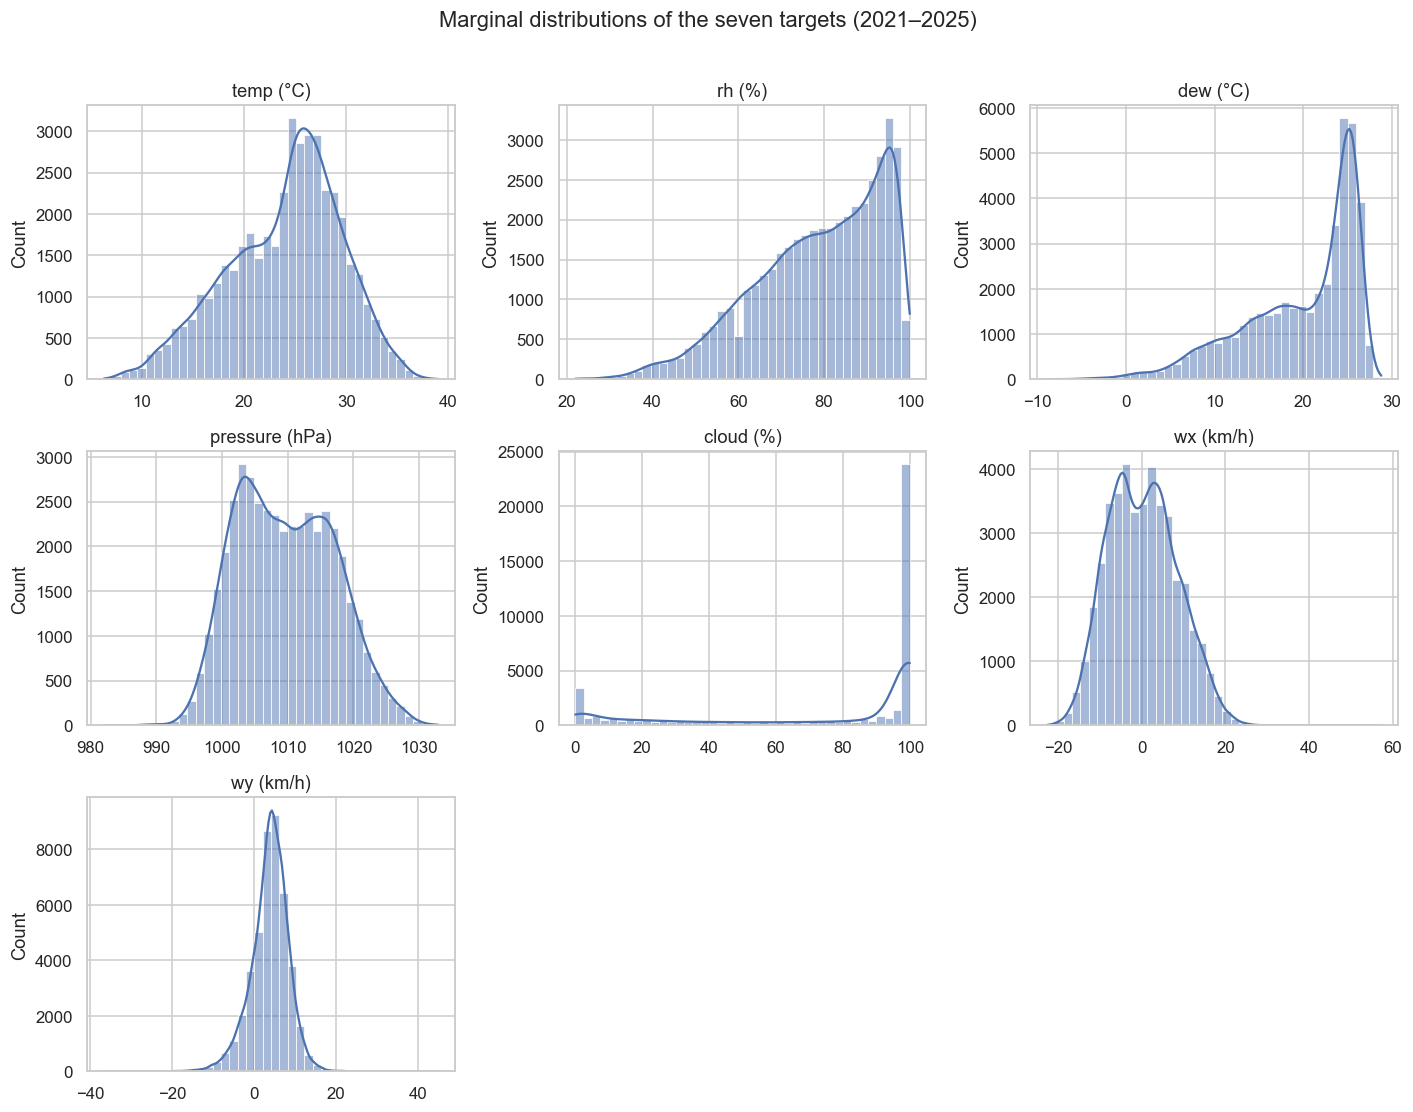
\includegraphics[width=\textwidth]{eda_hist.png}
\caption{Marginal distributions of the seven targets.}
\label{fig:eda-hist}
\end{figure}

\begin{figure}[H]\centering
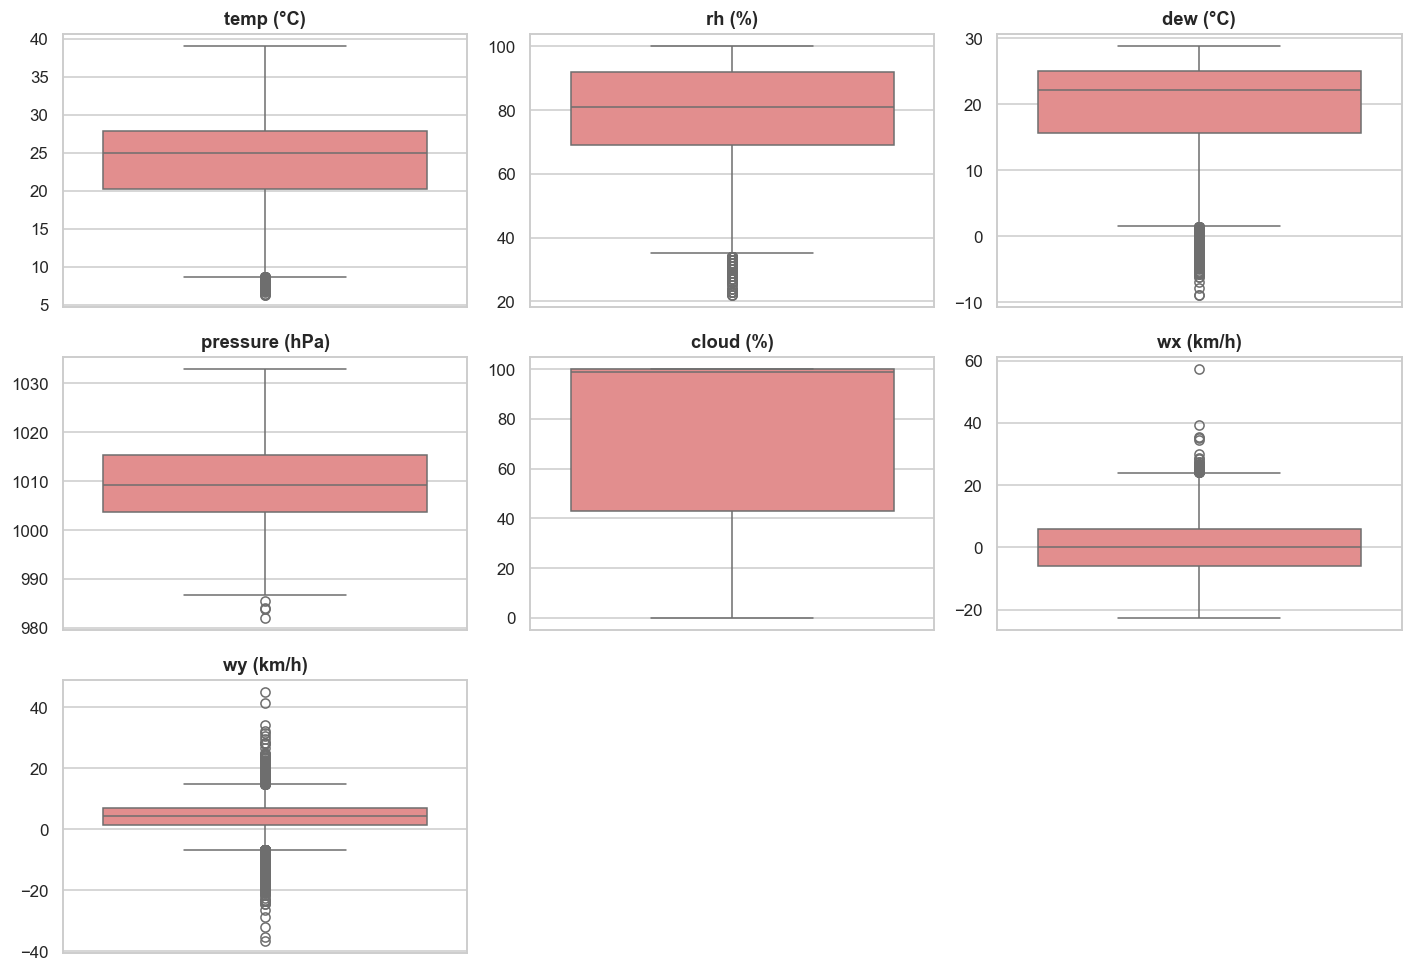
\includegraphics[width=0.95\textwidth]{eda_box.png}
\caption{Per-variable boxplots of the seven targets for outlier inspection.}
\label{fig:eda-box}
\end{figure}

\section{Correlation Analysis}
The correlation matrix (Fig.~\ref{fig:eda-corr}) reveals strong, physically
sensible dependencies: \texttt{temp}--\texttt{dew} ($+0.85$),
\texttt{dew}--\texttt{pressure} ($-0.87$), and \texttt{temp}--\texttt{pressure}
($-0.81$). Relative humidity correlates moderately with dew point ($+0.52$), while
\texttt{cloud} and the wind components are only weakly linearly related to the other
targets --- an early indication that \texttt{cloud} and wind will be the hardest to
forecast. These inter-variable links justify a \emph{multivariate} approach and the
lag/rolling features used by XGBoost.

\begin{figure}[H]\centering
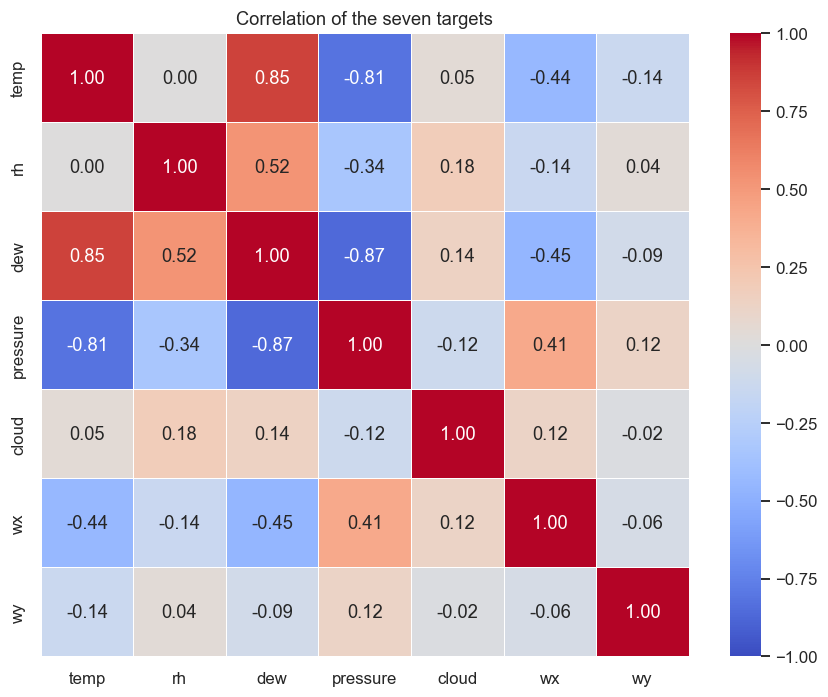
\includegraphics[width=0.8\textwidth]{eda_corr.png}
\caption{Correlation matrix of the seven targets.}
\label{fig:eda-corr}
\end{figure}

\section{Temporal Analysis}
Weekly means (Fig.~\ref{fig:eda-temporal}) show a clear annual cycle in
temperature and humidity and a milder seasonal swing in pressure. Aggregating by
month and by hour-of-day (Fig.~\ref{fig:eda-monthly}) exposes two dominant
periodicities: a seasonal cycle across the year and a strong diurnal cycle
(afternoon maximum, pre-dawn minimum). These two cycles directly motivate the
cyclical hour-of-day and day-of-year encodings in Chapter~\ref{ch:preprocess}.

\begin{figure}[H]\centering
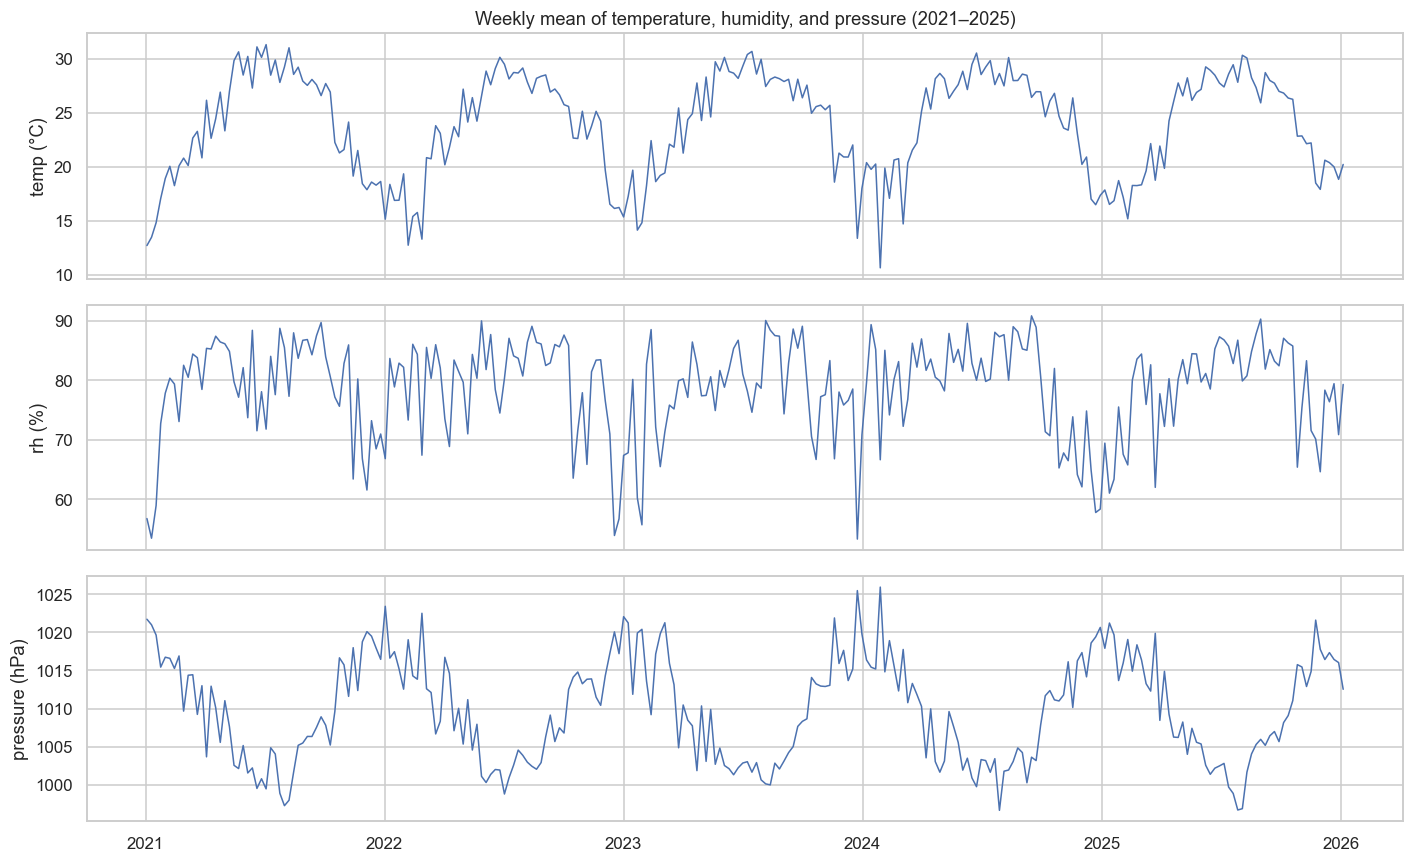
\includegraphics[width=\textwidth]{eda_temporal.png}
\caption{Weekly mean of temperature, humidity, and pressure over the full period.}
\label{fig:eda-temporal}
\end{figure}

\begin{figure}[H]\centering
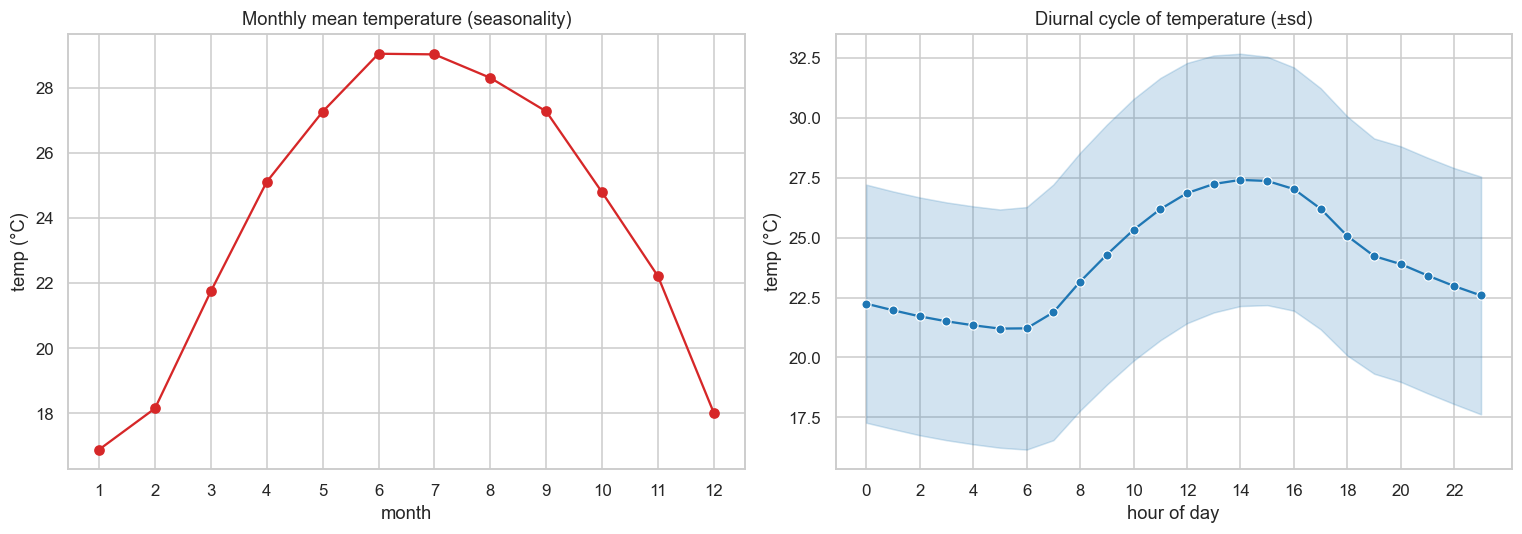
\includegraphics[width=\textwidth]{eda_monthly_diurnal.png}
\caption{Monthly seasonality (left) and diurnal cycle (right) of temperature.}
\label{fig:eda-monthly}
\end{figure}

\section{Target Variable Analysis}
An additive seasonal decomposition of daily-mean temperature
(Fig.~\ref{fig:eda-decomp}, period $=365$ days) separates a dominant annual
seasonal component (amplitude $\approx \pm5\,^\circ$C) from a slow trend and a
small residual. The large, regular seasonal term confirms that much of the
variance in the targets is predictable structure, which all models should
capture; the residual term bounds the irreducible short-term noise.

\begin{figure}[H]\centering
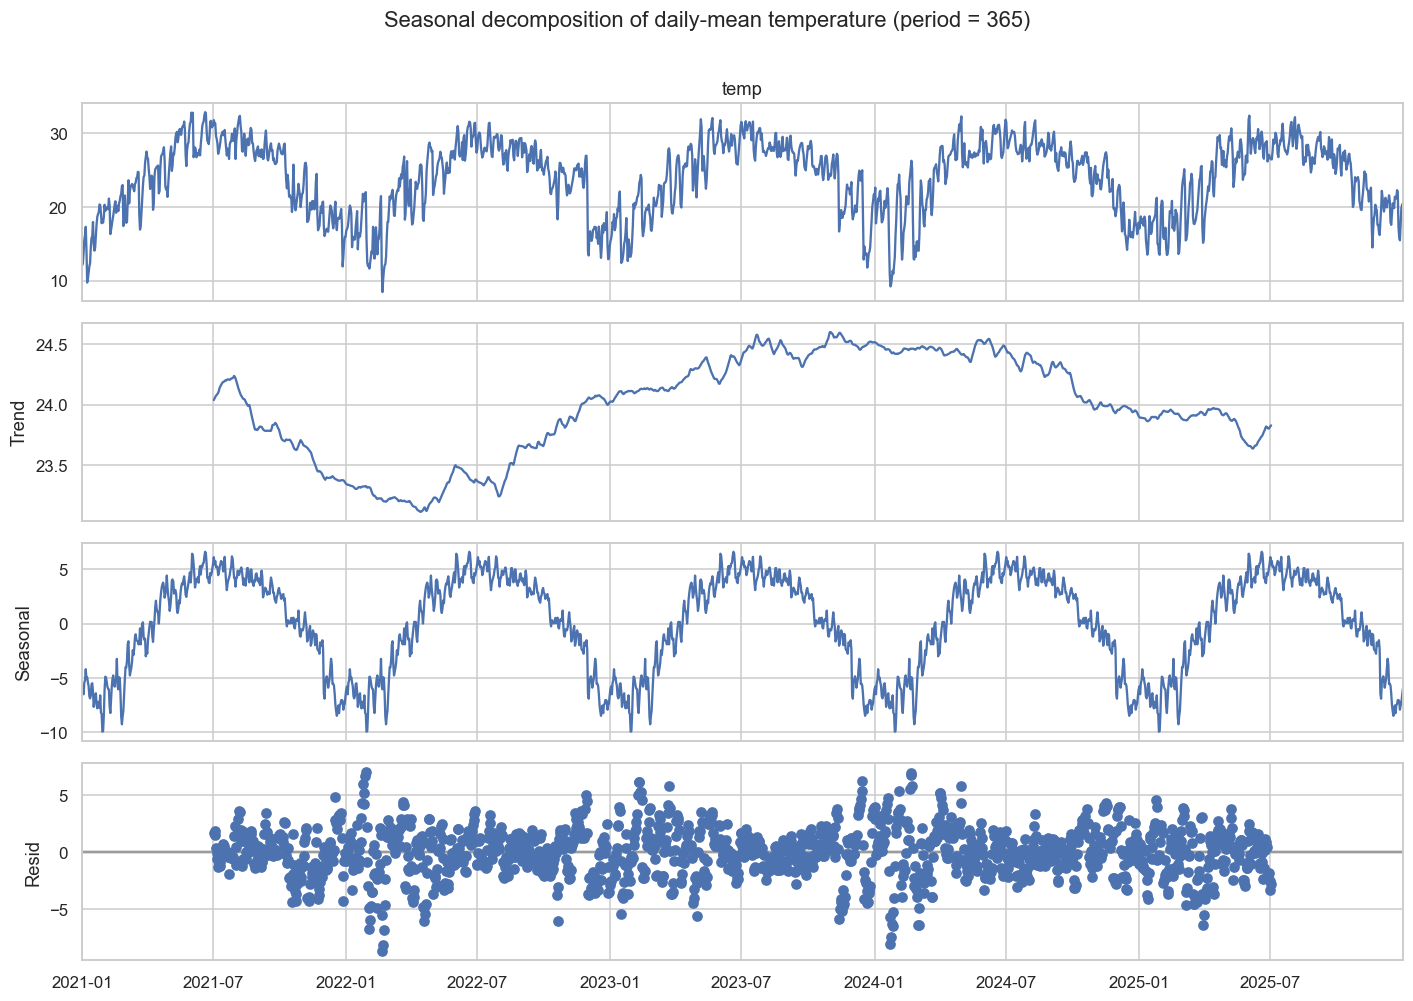
\includegraphics[width=\textwidth]{eda_decomp_temp.png}
\caption{Seasonal decomposition of daily-mean temperature.}
\label{fig:eda-decomp}
\end{figure}

Extending this to all seven targets (Fig.~\ref{fig:eda-decomp-all}) shows that each
variable carries a clear annual seasonal component: humidity and cloud cover have the
largest annual swings, the wind components the smallest, and every trend term is mild
and non-monotonic. The bulk of each series is therefore predictable seasonal
structure on top of short-term noise.

\begin{figure}[H]\centering
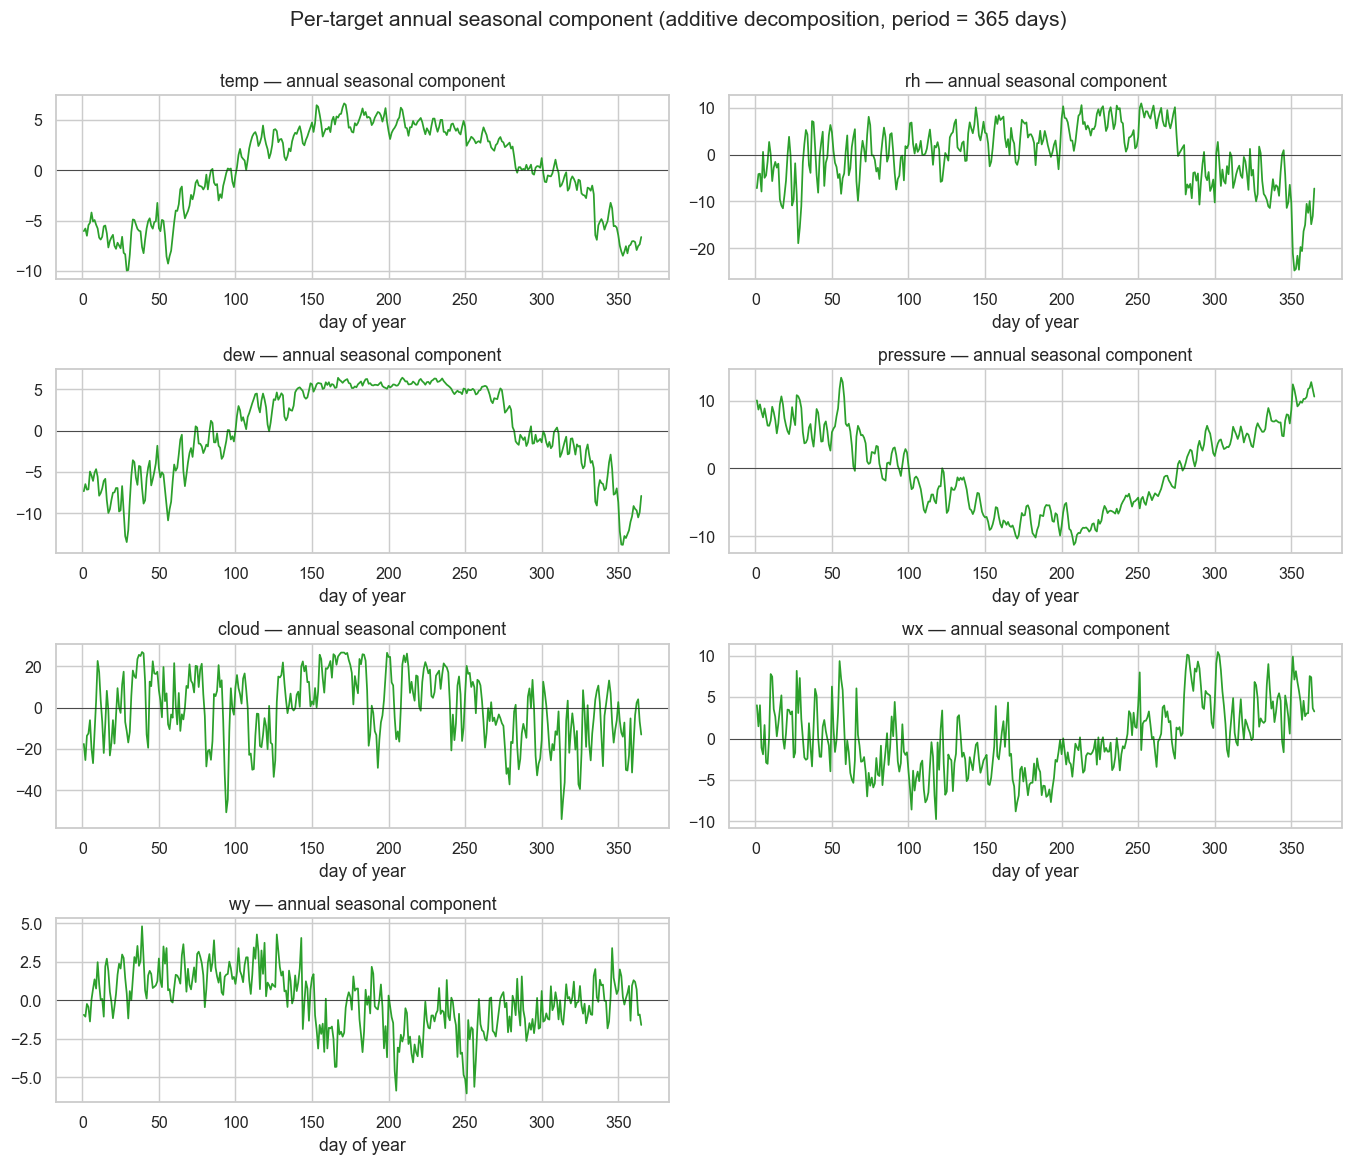
\includegraphics[width=\textwidth]{eda_decomp_all.png}
\caption{Annual seasonal component of each target (additive decomposition, period $=365$ days).}
\label{fig:eda-decomp-all}
\end{figure}

\section{Time-Series Structure}
\label{sec:eda-tsstruct}
This section adds the time-series diagnostics that directly inform the statistical
models (especially VAR, Section~\ref{sec:var}): stationarity, autocorrelation
structure, the diurnal cycle, and lagged cross-dependence.

\subsection{Stationarity}
Two complementary tests are applied to each target: the Augmented Dickey--Fuller
(ADF) test, whose null hypothesis is a unit root (small $p$ $\Rightarrow$
stationary), and the KPSS test, whose null hypothesis is stationarity (large $p$
$\Rightarrow$ stationary). Using both guards against the weaknesses of either alone.
The results (Table~\ref{tab:eda-adfkpss}) show that ADF rejects the unit root for all
seven targets at $p \le 10^{-12}$, and KPSS agrees (fails to reject stationarity) for
five of them. For \texttt{temp} and \texttt{wx}, KPSS marginally rejects
($p = 0.049$ and $0.030$); combined with the decisive ADF rejection, this points to
\emph{deterministic} annual seasonality rather than a stochastic trend --- a pattern
also visible as the wavy-but-flat rolling mean in Fig.~\ref{fig:eda-rolling}, whose
rolling standard deviation stays roughly constant. Differencing is therefore not
required, justifying the $d=0$ choice used by the VAR model.

\begin{table}[H]\centering
\caption{Stationarity tests on the seven targets (full 2021--2025 series).}
\label{tab:eda-adfkpss}
\begin{tabular}{lccl}
\toprule
\textbf{Variable} & \textbf{ADF $p$} & \textbf{KPSS $p$} & \textbf{Verdict} \\
\midrule
\texttt{temp}     & $6.6\times10^{-13}$ & $0.049$      & stationary (borderline KPSS: annual cycle) \\
\texttt{rh}       & $4.3\times10^{-29}$ & $\ge 0.10$   & stationary \\
\texttt{dew}      & $2.1\times10^{-14}$ & $\ge 0.10$   & stationary \\
\texttt{pressure} & $6.5\times10^{-13}$ & $\ge 0.10$   & stationary \\
\texttt{cloud}    & $<10^{-30}$         & $\ge 0.10$   & stationary \\
\texttt{wx}       & $2.9\times10^{-30}$ & $0.030$      & stationary (borderline KPSS: annual cycle) \\
\texttt{wy}       & $<10^{-30}$         & $\ge 0.10$   & stationary \\
\bottomrule
\end{tabular}
\end{table}

\begin{figure}[H]\centering
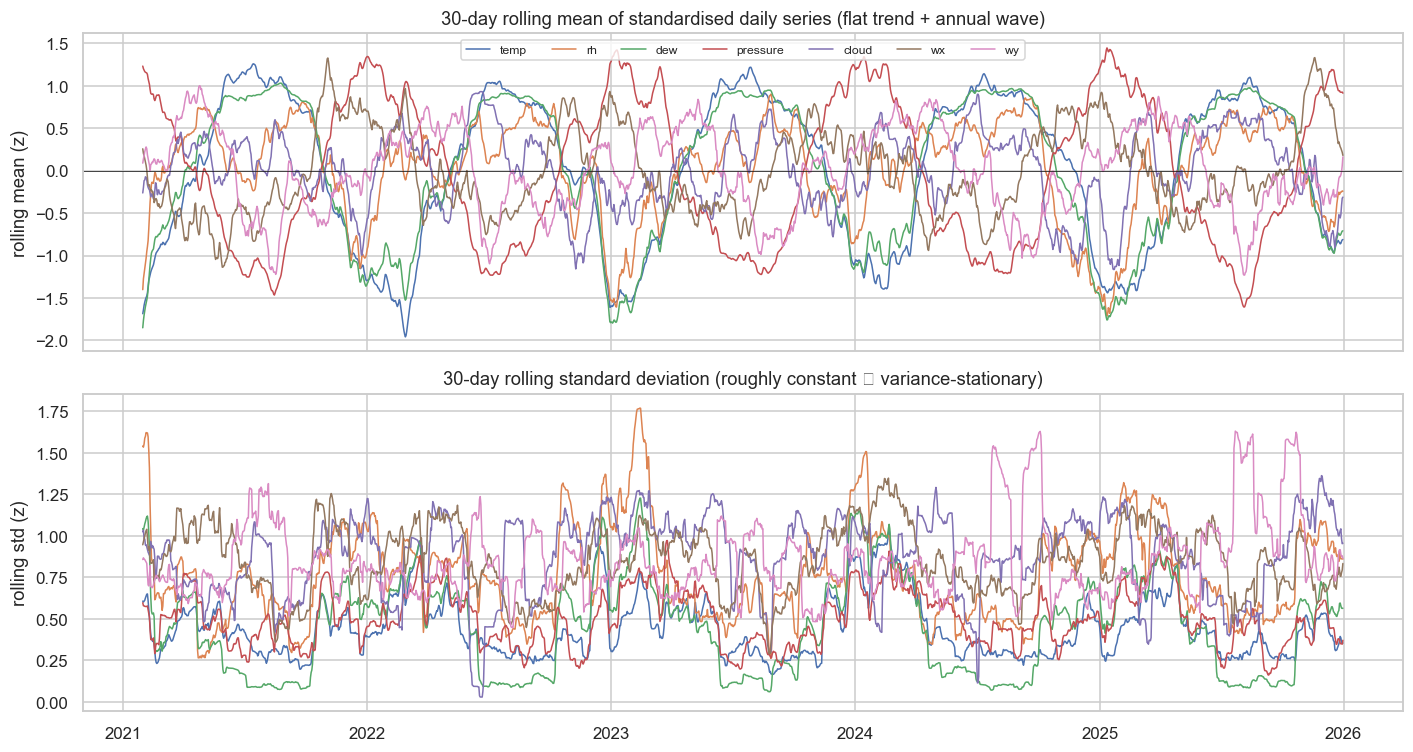
\includegraphics[width=\textwidth]{eda_rolling.png}
\caption{Rolling 30-day mean and standard deviation of the standardised daily series.
The mean is flat apart from an annual wave (seasonality, not a unit-root trend) and
the standard deviation is roughly constant.}
\label{fig:eda-rolling}
\end{figure}

\subsection{Autocorrelation Structure}
The autocorrelation (ACF) and partial-autocorrelation (PACF) functions
(Fig.~\ref{fig:eda-acfpacf}) characterise each target's memory. The ACFs decay slowly
with a clear periodic bump near lag $24$ (the daily cycle), while the PACFs cut off
after a few lags, with an additional spike near lag $24$. This ``PACF cuts off,
ACF tails off'' signature indicates an autoregressive structure of low base order plus
daily-cycle lags, and cross-checks the AIC-selected lag order used by VAR
(Section~\ref{sec:var-train}).

\begin{figure}[H]\centering
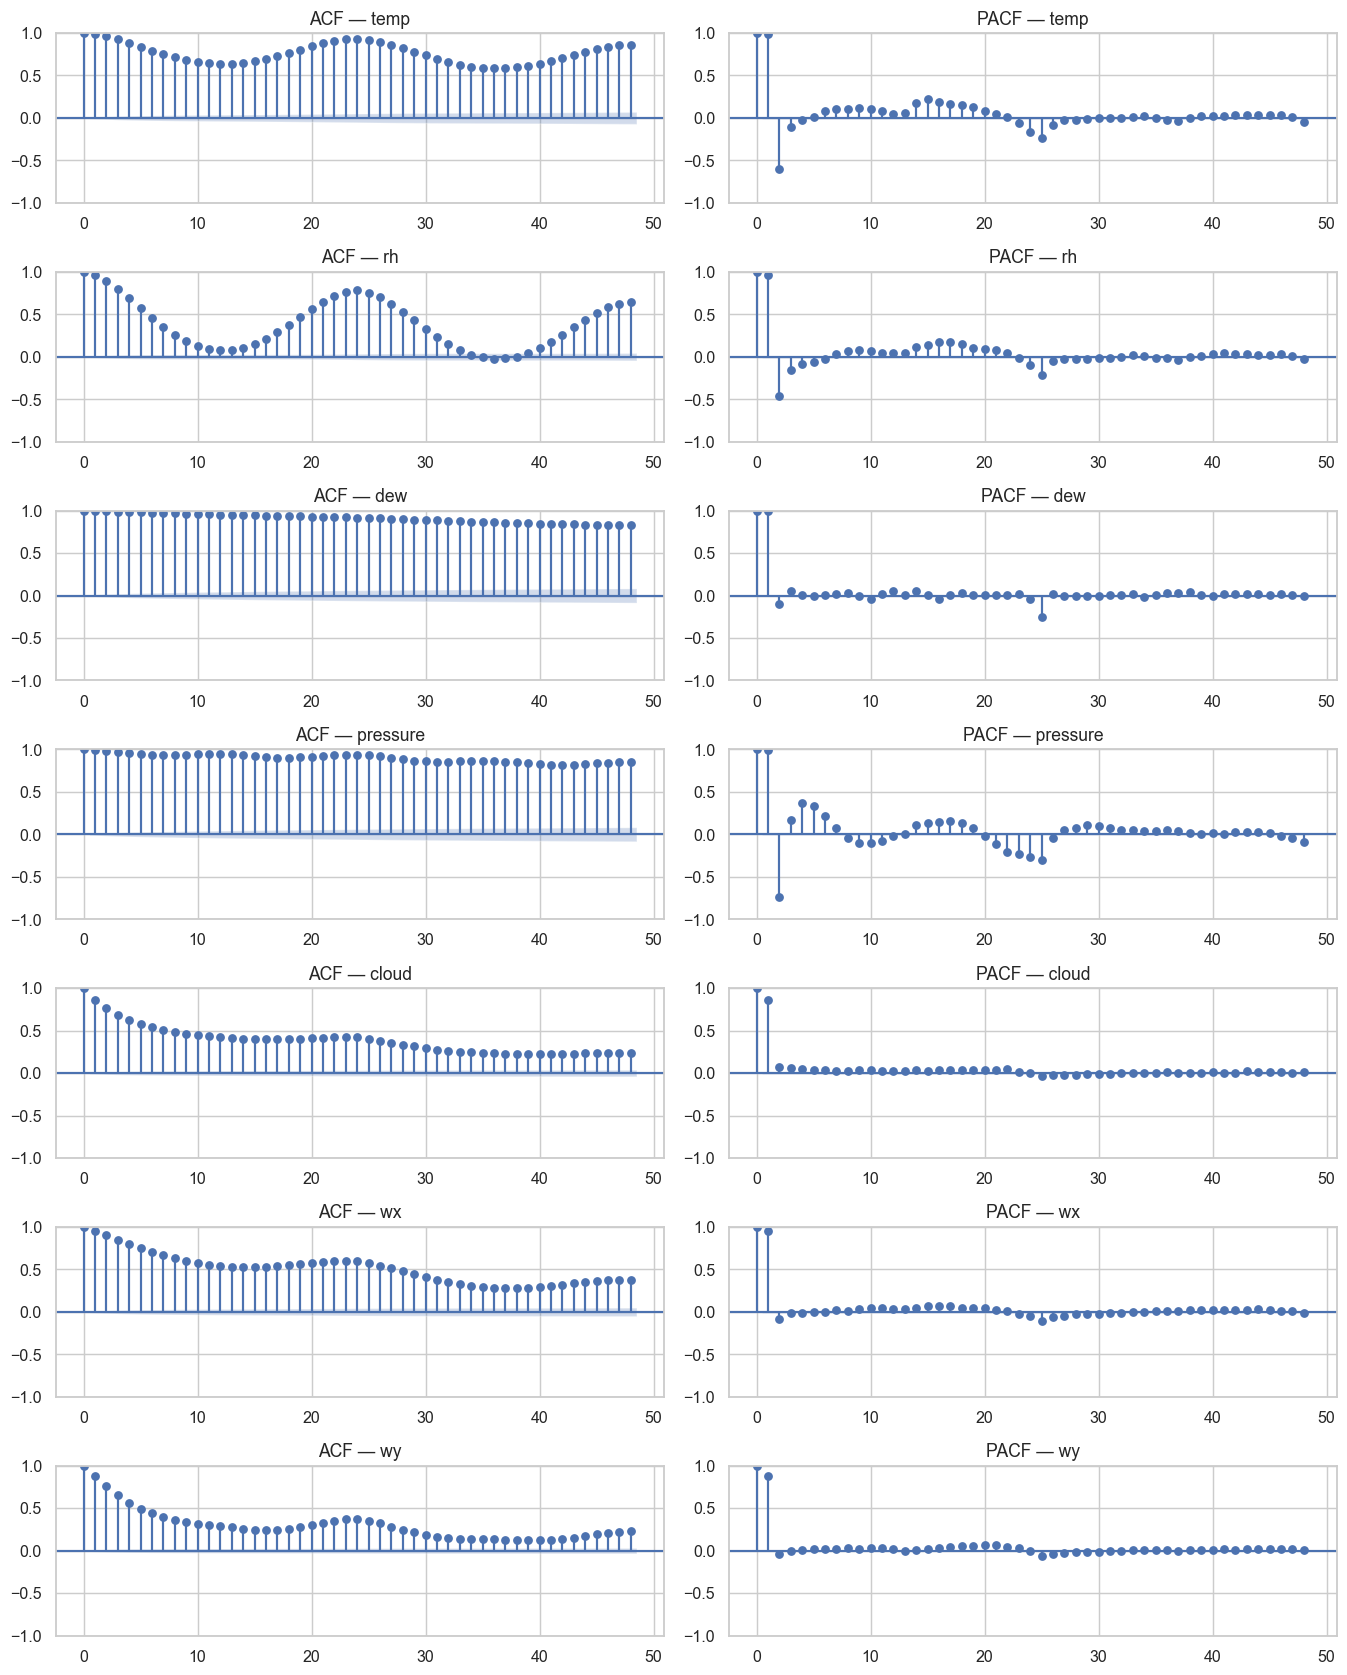
\includegraphics[width=0.92\textwidth]{eda_acf_pacf.png}
\caption{ACF (left) and PACF (right) of each target, lags $0$--$48$ hours.}
\label{fig:eda-acfpacf}
\end{figure}

\subsection{Diurnal Cycle}
Standardising each target by hour of day (Fig.~\ref{fig:eda-daily-cycle}) exposes the
$24$-hour cycle directly: \texttt{temp} peaks in the afternoon and troughs before
dawn, \texttt{rh} moves in near-perfect anti-phase, and the wind components show a
clear daytime/nighttime pattern, whereas \texttt{cloud} and \texttt{pressure} have
weaker, phase-shifted cycles. The afternoon temperature peak near $07$--$08$h on the
$x$-axis indicates the timestamps are in UTC for this location.

\begin{figure}[H]\centering
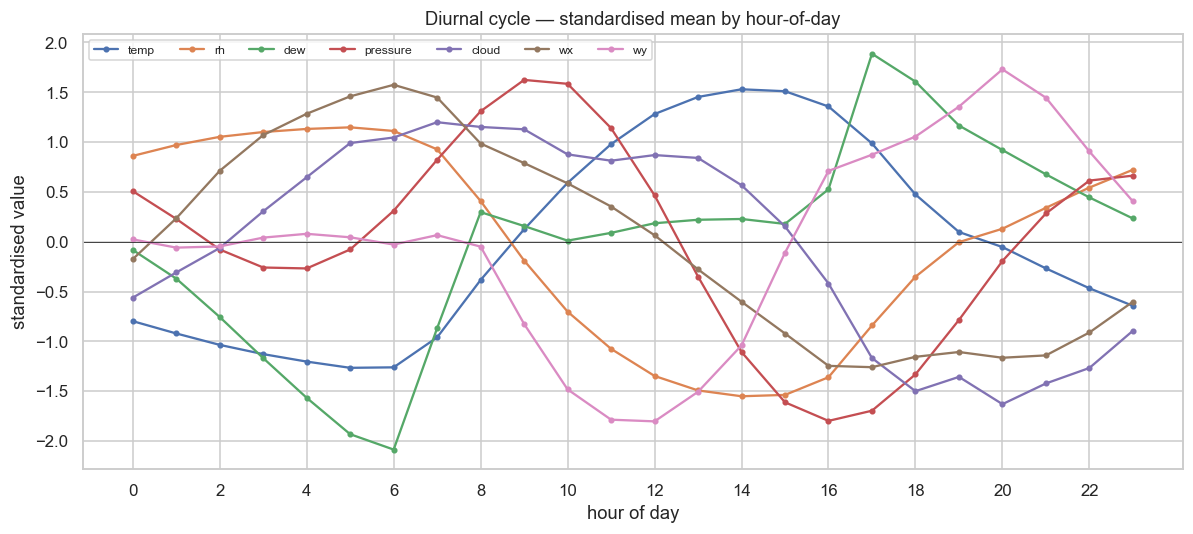
\includegraphics[width=0.85\textwidth]{eda_daily_cycle.png}
\caption{Diurnal cycle: standardised mean of each target by hour of day.}
\label{fig:eda-daily-cycle}
\end{figure}

\subsection{Lagged Cross-Correlation}
Finally, the lagged cross-correlation matrix (Fig.~\ref{fig:eda-crosscorr}) measures
how each target's recent past ($t-3$\,h) relates to each other target's present.
Strong off-diagonal entries appear among the thermodynamic variables ---
\texttt{dew}--\texttt{pressure} ($-0.87$), \texttt{temp}--\texttt{dew} ($+0.85$), and
\texttt{temp}--\texttt{pressure} ($-0.84$) --- meaning one variable's history carries
predictive information about another. This lagged cross-dependence is exactly the
signal a \emph{multivariate} model (VAR) can exploit but seven independent univariate
models cannot, and it motivates the multivariate approach taken throughout this study.

\begin{figure}[H]\centering
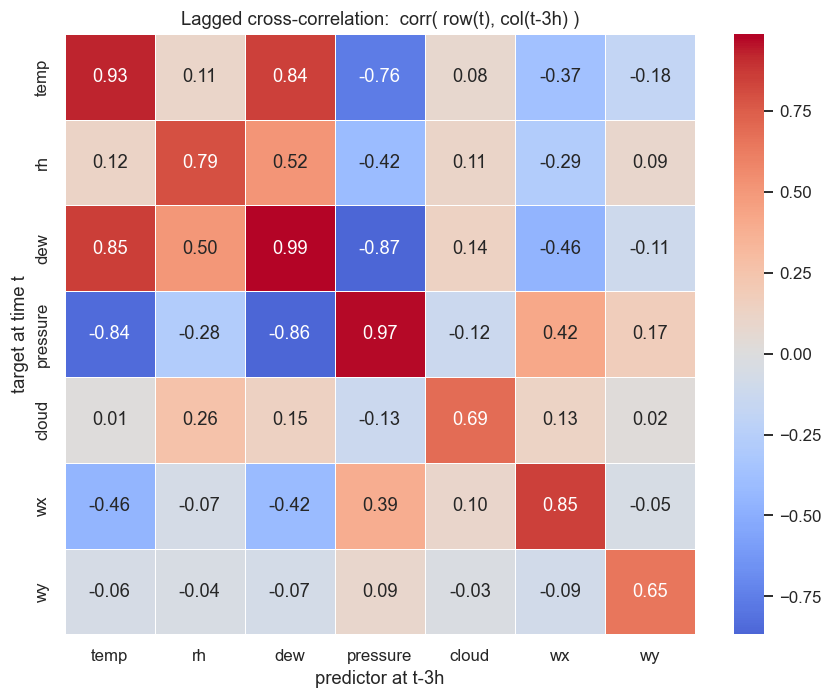
\includegraphics[width=0.72\textwidth]{eda_crosscorr.png}
\caption{Lagged cross-correlation $\mathrm{corr}\big(\mathrm{row}(t),\,\mathrm{col}(t-3\text{h})\big)$ among the seven targets.}
\label{fig:eda-crosscorr}
\end{figure}

\section{Key Findings from EDA}
\begin{itemize}
  \item \textbf{Complete data} --- no missing values or gaps, so no imputation is
        needed (Chapter~\ref{ch:preprocess} interpolation is a safeguard only).
  \item \textbf{Strong periodicity} --- pronounced annual and diurnal cycles
        $\Rightarrow$ cyclical time encodings are added as input features.
  \item \textbf{Strong inter-variable correlation} (temp/dew/pressure)
        $\Rightarrow$ a multivariate model with lagged cross-features is
        appropriate.
  \item \textbf{Skewed/bounded targets} --- \texttt{cloud} is bimodal and the wind
        components \texttt{wx}/\texttt{wy} take zero/near-zero values when calm
        $\Rightarrow$ MAPE is unsafe for these, MAE is the primary metric, and
        \texttt{cloud} is expected to be hardest.
  \item \textbf{Genuine extremes} in the wind components $\Rightarrow$ retained
        (not clipped, except the non-negativity guard on wind speed).
  \item \textbf{Stationary in levels} --- ADF and KPSS agree the targets have no
        unit root (Table~\ref{tab:eda-adfkpss}); the borderline KPSS cases reflect
        deterministic annual seasonality $\Rightarrow$ no differencing ($d=0$).
  \item \textbf{Low AR order + daily lag} --- the PACF cuts off after a few lags with
        a lag-$24$ spike $\Rightarrow$ a modest lag order augmented by daily-cycle
        terms suffices (cross-checks the AIC choice for VAR).
  \item \textbf{Lagged cross-dependence} --- strong off-diagonal cross-correlations
        among \texttt{temp}/\texttt{dew}/\texttt{pressure}
        (Fig.~\ref{fig:eda-crosscorr}) $\Rightarrow$ a multivariate model can exploit
        structure unavailable to univariate ones.
\end{itemize}

%==============================================================================
\chapter{Data Preprocessing}
\label{ch:preprocess}

The same preprocessing is applied to every model so the comparison is fair.

\section{Data Cleaning}
The \texttt{time} column is parsed to a timestamp, set as the index, sorted
ascending, and resampled to a strict hourly frequency. As a sensor-error guard,
wind speed is clipped to be non-negative,
\[
  \texttt{wind\_speed} \leftarrow \max(\texttt{wind\_speed}, 0),
\]
which removes spurious sentinel values (e.g.\ $-9999$).

\section{Missing Value Handling}
Any incidental gaps are filled by time-based interpolation followed by forward-
and back-filling:
\[
  \tilde{x}_t = \operatorname{interp}(x)_t, \qquad
  \text{then } \texttt{ffill} \to \texttt{bfill}.
\]
On the present dataset there are no gaps, so this step is a safeguard.

\section{Wind Decomposition}
Wind direction is circular and not directly learnable; it is converted to
Cartesian components,
\begin{align}
  \texttt{wx} &= \texttt{wind\_speed} \cdot \cos\!\big(\operatorname{rad}(\texttt{wind\_dir})\big), \\
  \texttt{wy} &= \texttt{wind\_speed} \cdot \sin\!\big(\operatorname{rad}(\texttt{wind\_dir})\big),
\end{align}
so that magnitude and direction are encoded smoothly.

\section{Cyclical Time Encoding}
Hour-of-day and day-of-year are encoded with sine/cosine pairs to respect their
periodicity:
\begin{align}
  \text{hour}_{\sin} &= \sin\!\Big(\tfrac{2\pi\, h}{24}\Big), &
  \text{hour}_{\cos} &= \cos\!\Big(\tfrac{2\pi\, h}{24}\Big), \\
  \text{doy}_{\sin}  &= \sin\!\Big(\tfrac{2\pi\, d}{365.25}\Big), &
  \text{doy}_{\cos}  &= \cos\!\Big(\tfrac{2\pi\, d}{365.25}\Big).
\end{align}

\section{Feature Scaling}
A \texttt{StandardScaler} is fit on the \emph{training partition only} and applied
to validation and test:
\[
  z = \frac{x - \mu_{\text{train}}}{\sigma_{\text{train}}}.
\]
All forecasts are inverted to the real scale before any metric is computed.
Tree models are scale-invariant; scaling is retained for protocol consistency
with the deep-learning models.

\section{Train/Validation/Test Split}
The split is strictly chronological and never shuffled (Table~\ref{tab:split}).

\begin{table}[H]
\centering
\caption{Chronological data split.}
\label{tab:split}
\begin{tabular}{llrl}
\toprule
\textbf{Split} & \textbf{Years} & \textbf{Hours} & \textbf{Role} \\
\midrule
Train & 2021--2023 & 26{,}280 & Fit model parameters \\
Val   & 2024       &  8{,}784 & Tuning / early stopping \\
Test  & 2025       &  8{,}760 & Final evaluation (untouched) \\
\bottomrule
\end{tabular}
\end{table}

\section{Sliding-Window Generation}
For machine-/deep-learning models, the series is converted to supervised windows:
an input lookback of $L = 120$ hours predicts the next $H = 24$ hours,
\[
  \underbrace{\mathbf{X} \in \mathbb{R}^{L \times d_{\text{in}}}}_{\text{input window}}
  \;\longrightarrow\;
  \underbrace{\mathbf{Y} \in \mathbb{R}^{H \times 7}}_{\text{forecast block}} .
\]
Forecasts only ever condition on observations strictly before the target window,
preventing leakage.

\section{Feature Engineering Overview}
Tree models cannot exploit a raw flattened window effectively, so each
$(120, d_{\text{in}})$ window is summarised into a compact feature vector
(recent lags and rolling statistics per channel). Every engineered feature is a
function of the 120-hour history up to the origin, preserving the same
no-leakage horizon as the raw window. The full construction is detailed in
Section~\ref{sec:xgb-fe}.

%==============================================================================
\chapter{Forecasting Models}
\label{ch:models}


% ================================================================

% ================================================================

\section{DLinear}
\label{sec:dlinear}

\subsection{Overview}

DLinear \citep{zeng2023dlinear} is a decomposition-based linear model that
challenges the prevailing trend of applying complex Transformer architectures
to time series forecasting. The core insight is that a time series can be
separated into a slow-moving trend and a fast-moving seasonal component, each
forecast independently with a single linear layer, then recombined. Despite
extreme simplicity --- only 5,892 parameters for the shared-weight variant ---
DLinear matches or exceeds state-of-the-art Transformers on standard benchmarks
while training orders of magnitude faster.

In this project, DLinear is applied as a \textbf{multivariate multi-step}
forecaster: a single model consumes the full $120 \times 11$ input window
(7 weather channels + 4 cyclical time encodings) and outputs a $24 \times 7$
forecast block covering all seven protocol targets simultaneously. A final linear
projection layer maps the 11 input channels to the 7 output targets, allowing the
model to exploit cross-variable dependencies learned from data.

Two variants are evaluated:
\begin{itemize}
  \item \textbf{DLinear-S} (Shared): one pair of trend/seasonal linear layers
        shared across all 11 input channels --- 5,892 parameters.
  \item \textbf{DLinear-I} (Individual): per-channel trend/seasonal linear
        layers --- 63,972 parameters.
\end{itemize}

% ---------------------------------------------------------------
\subsection{Mathematical Formulation}
% ---------------------------------------------------------------

Let $\mathbf{X} \in \mathbb{R}^{L \times C_{\text{in}}}$ be an input window of
$L = 120$ hours and $C_{\text{in}} = 11$ features (7 weather variables + 4
cyclical time encodings). The model produces
$\mathbf{\hat{Y}} \in \mathbb{R}^{H \times C_{\text{out}}}$ with $H = 24$ hours
and $C_{\text{out}} = 7$ target variables.

\subsubsection{Series Decomposition}

A 1D average pooling with kernel size $k = 25$ and stride 1 extracts the trend
while preserving sequence length. For a sequence of length $L$, the first and
last time steps are replicated $p = (k-1)/2 = 12$ times and concatenated to both
ends before pooling --- a technique called \textbf{replication padding} used by
the official implementation \citep{zeng2023dlinear}:
%
\begin{equation}
\mathbf{X}_{\text{padded}} = [\,\underbrace{\mathbf{X}_0, \ldots, \mathbf{X}_0}_{p \text{ times}},\;
        \mathbf{X}_0, \ldots, \mathbf{X}_{L-1},\;
        \underbrace{\mathbf{X}_{L-1}, \ldots, \mathbf{X}_{L-1}}_{p \text{ times}}\,]
        \quad \in \mathbb{R}^{(L + 2p) \times C_{\text{in}}}
\end{equation}
%
\begin{equation}
\mathbf{T} = \text{AvgPool1d}\big(\mathbf{X}_{\text{padded}},\;
            \text{kernel}=k,\; \text{padding}=0\big)
            \quad \in \mathbb{R}^{L \times C_{\text{in}}}
\end{equation}
%
\begin{equation}
\mathbf{S} = \mathbf{X} - \mathbf{T} \quad \in \mathbb{R}^{L \times C_{\text{in}}}
\end{equation}
%
At each position $t$, the trend is the unweighted mean of the $k$ values in the
local window:
%
\begin{equation}
\mathbf{T}_t = \frac{1}{k} \sum_{j=t-p}^{t+p} \mathbf{X}_{\text{padded}, j}
\end{equation}

The kernel size $k=25$ spans just over one full diurnal cycle (24 h), causing
the day--night oscillation to approximately cancel when averaged, leaving only
the multi-day trend. The seasonal component $\mathbf{S}$ captures all remaining
variation: diurnal cycles, short-term fluctuations, and noise.

\paragraph{Why replication padding.}
At the boundaries ($t < p$ and $t \ge L-p$), the kernel extends beyond available
data. Repeating the boundary values --- rather than padding with zeros ---
encodes a \textbf{persistence} assumption: if nothing is known beyond the edge,
the most conservative guess is that conditions remain unchanged. Concretely, at
the leftmost position:
%
\begin{equation}
\mathbf{T}_0 = \frac{\overbrace{\mathbf{X}_0 + \cdots + \mathbf{X}_0}^{p+1 \text{ times}}
        + \mathbf{X}_1 + \cdots + \mathbf{X}_p}{k}
        = \frac{(p+1)\,\mathbf{X}_0 + \sum_{j=1}^{p} \mathbf{X}_j}{k}
\end{equation}
%
All $k=25$ positions in the kernel contain real observations or faithful copies;
no position is underweighted. The first and last 12 positions (24 of 120 h, 20\%
of the lookback window) are affected; the rightmost 12 are the hours closest to
the forecast origin, where the signal is most informative for short-horizon
prediction.

\subsubsection{Dual Linear Projection}

Each component is independently mapped from the 120 h lookback to the 24 h
forecast horizon via a single linear layer:
%
\begin{align}
\mathbf{\hat{Y}}_t &= \mathbf{W}_t \, \mathbf{T} + \mathbf{b}_t
        \quad \in \mathbb{R}^{H \times C_{\text{in}}}
        \qquad \text{(Trend forecast)} \\
\mathbf{\hat{Y}}_s &= \mathbf{W}_s \, \mathbf{S} + \mathbf{b}_s
        \quad \in \mathbb{R}^{H \times C_{\text{in}}}
        \qquad \text{(Seasonal forecast)}
\end{align}
%
where $\mathbf{W}_t, \mathbf{W}_s \in \mathbb{R}^{H \times L}$ and
$\mathbf{b}_t, \mathbf{b}_s \in \mathbb{R}^{H}$.

\begin{itemize}
  \item \textbf{DLinear-S}: a single pair $(\mathbf{W}_t, \mathbf{W}_s)$ is
        shared across all $C_{\text{in}}$ channels.
  \item \textbf{DLinear-I}: each channel $c \in \{1, \ldots, C_{\text{in}}\}$
        has its own pair $\mathbf{W}_t^{(c)}, \mathbf{W}_s^{(c)} \in
        \mathbb{R}^{H \times L}$, implemented as $C_{\text{in}}$ separate
        \texttt{nn.Linear(L, H)} modules.
\end{itemize}

\subsubsection{Combine and Project}
%
\begin{align}
\mathbf{\hat{Y}}_{\text{raw}} &= \mathbf{\hat{Y}}_t + \mathbf{\hat{Y}}_s
        \quad \in \mathbb{R}^{H \times C_{\text{in}}} \\
\mathbf{\hat{Y}} &= \mathbf{\hat{Y}}_{\text{raw}} \, \mathbf{W}_{\text{proj}}
        \quad \in \mathbb{R}^{H \times C_{\text{out}}}
\end{align}
%
$\mathbf{W}_{\text{proj}} \in \mathbb{R}^{C_{\text{in}} \times C_{\text{out}}}$
maps the $C_{\text{in}}$ input channels to the $C_{\text{out}}$ protocol targets.
This projection is linear and data-driven: the model learns weighted combinations
of input channels for each target variable (e.g.\ $wx$ and $wy$ may contribute to
predicting each other, temperature helps predict dew point).

\textbf{Parameter count:}
\begin{itemize}
  \item DLinear-S: $2 \times (LH + H) \times 1 + C_{\text{in}} C_{\text{out}}
        = \mathbf{5{,}892}$
  \item DLinear-I: $2 \times (LH + H) \times C_{\text{in}} + C_{\text{in}}
        C_{\text{out}} = \mathbf{63{,}972}$
\end{itemize}

\subsubsection{Why Decomposition Helps}

The decomposition acts as an \textbf{inductive bias}. The trend branch only needs
to learn a smooth continuation (``is it getting warmer or cooler over the next 24
hours?''), while the seasonal branch only needs to capture the repeating diurnal
pattern (``at what hour does the daily peak occur?''). By separating these two
structurally different tasks, each linear layer solves a simpler problem than one
layer would face on the raw mixed signal.

\textbf{Concrete example (first 48 h of 2021, temperature):}
\begin{table}[H]
\centering
\caption{Decomposition of the first 48 hours of temperature (2021).}
\begin{tabular}{lll}
\toprule
Component & Value range & Meaning \\
\midrule
Raw temp  & $9.4 \to 18.1$\,°C & Day--night oscillation on warming trend \\
Trend ($k=25$) & $5.4 \to 11.4$\,°C & Smooth multi-day warming of $\sim$6\,°C \\
Seasonal & $+4.0$ at noon, $-3.0$ at midnight & Clean 24 h cycle, $\sim\pm 5$\,°C amplitude \\
\bottomrule
\end{tabular}
\end{table}

% ---------------------------------------------------------------
\subsection{Pipeline Overview}
% ---------------------------------------------------------------

Figure~\ref{fig:dlinear-pipeline} shows the end-to-end DLinear pipeline from raw
CSV to final evaluation.

\begin{figure}[H]
\centering
\fbox{%
\begin{tabular}{cccccc}
\toprule
\textbf{CSV} & \textbf{Preprocess} & \textbf{Window} & \textbf{Train} &
\textbf{Eval} & \textbf{Diag} \\
43,824 rows & $\rightarrow$ & 120$\to$24 & $\rightarrow$ & 360 origins & $\rightarrow$ \\
14 cols
  & $\bullet$ clip
  & sliding
  & $\bullet$ Adam
  & (2025)
  & $\bullet$ ADF \\
  & $\bullet$ wind$\to$wx,wy
  & 26,137 train
  & $\bullet$ early stop
  &
  & $\bullet$ LB \\
  & $\bullet$ sin/cos hour,doy
  &
  & $\bullet$ 3 seeds
  &
  & $\bullet$ Norm \\
  & $\bullet$ scaler
  &
  &
  &
  & $\bullet$ BS CI \\
\bottomrule
\end{tabular}}
\caption{DLinear end-to-end pipeline.}
\label{fig:dlinear-pipeline}
\end{figure}

The pipeline comprises five stages:
\begin{enumerate}
  \item \textbf{Preprocessing} --- parse time index, clip negative wind speeds
        (sensor-error guard), decompose wind direction to Cartesian components
        ($wx$, $wy$), interpolate any gaps, add 4 cyclical time encodings
        ($\sin$/$\cos$ of hour-of-day and day-of-year), apply StandardScaler
        fitted on train only.
  \item \textbf{Window generation} --- slide a 120 h lookback window across the
        series at stride 1 to produce $(X, Y)$ pairs of shape
        $(120, 11) \to (24, 7)$. Chronological split: 2021--2023 train, 2024
        val, 2025 test.
  \item \textbf{Training} --- feed windows through the DLinear model; optimize
        MSE with Adam and ReduceLROnPlateau; early-stop on validation loss.
        Three seeds trained per variant.
  \item \textbf{Evaluation} --- rolling-origin over 2025: advance origin in 24 h
        non-overlapping steps (360 origins), invert StandardScaler, compute
        MAE/RMSE overall, per-variable, and per-horizon.
  \item \textbf{Diagnostics} --- protocol \S6 checks: ADF stationarity,
        Ljung--Box residual autocorrelation, residual normality, empirical
        forecast intervals, bootstrap CIs, and training stability.
\end{enumerate}



% ---------------------------------------------------------------
\subsection{Training Procedure}
% ---------------------------------------------------------------

\textbf{One model, all targets.} Unlike XGBoost (which trains one regressor per
target), a single DLinear model predicts all seven targets jointly. The final
projection layer $\mathbf{W}_{\text{proj}}$ learns cross-target relationships
directly from the training data.

\textbf{Data usage.} The model trains on the full 2021--2023 sliding windows at
stride 1 (26,137 windows). Every window conditions strictly on observations
before the target horizon, preventing leakage. No subsampling or stride reduction
is applied --- the model is fast enough to use all available windows.

\textbf{Validation and early stopping.} Training minimizes MSE with the Adam
optimizer \citep{kingma2015adam}. A ReduceLROnPlateau scheduler halves the
learning rate when validation loss fails to improve for 5 epochs. Early stopping
terminates training when validation loss does not improve for 10 consecutive
epochs, capped at 50 epochs total. All hyperparameters
(Table~\ref{tab:dlinear-hparams}) are fixed a priori --- there is no grid search
--- and the 2025 test set is never seen during training.

\textbf{Convergence.} On an NVIDIA GeForce RTX 4060 GPU, DLinear-S converges in
$\sim$85 s per seed to a mean validation MSE of $0.3538 \pm 1.6\!\times\!10^{-4}$
(3 seeds). DLinear-I converges in $\sim$233 s per seed to
$0.3451 \pm 5.7\!\times\!10^{-4}$. Both plateau smoothly without divergence:
validation loss slopes over the last 10 epochs are $-1.5 \times 10^{-4}$ (S) and
$-3.6 \times 10^{-4}$ (I) --- both effectively flat. The train--validation loss
gap is small (S: $-0.030$; I: $-0.036$), indicating no overfitting.

\textbf{Multi-seed training.} Per protocol \S8, three seeds
$\{42, 123, 456\}$ are trained and checkpoints saved for each seed per variant.
The purely linear optimization landscape is near-convex, leading to highly
consistent convergence regardless of random initialization: across 3 seeds, MAE
standard deviation is $0.004$ for S and $0.023$ for I.

\begin{table}[H]
\centering
\caption{DLinear training hyperparameters.}
\label{tab:dlinear-hparams}
\begin{tabular}{ll}
\toprule
\textbf{Parameter} & \textbf{Value} \\
\midrule
Optimizer      & Adam \\
Learning rate  & $10^{-3}$ \\
Weight decay   & $10^{-5}$ \\
Loss           & MSE \\
Batch size     & 64 \\
LR scheduler   & ReduceLROnPlateau (factor 0.5, patience 5) \\
Early stopping & Patience 10 epochs, max 50 \\
Kernel size    & 25 \\
Seeds          & $\{42, 123, 456\}$ \\
\bottomrule
\end{tabular}
\end{table}

% ---------------------------------------------------------------
\subsection{Algorithm}
% ---------------------------------------------------------------

\begin{spacing}{1.0}
\begin{algorithm}[H]
\small
\caption{DLinear training and rolling-origin evaluation}
\label{alg:dlinear}
\begin{algorithmic}[1]
\Require Hourly series $S[0..T]$; $L=120$; $H=24$; $V=7$; $k=25$;
         seeds $\{42,123,456\}$
\State \textbf{Preprocess:}
\State \quad Parse time; clip wind $\ge 0$
\State \quad $wx = \text{speed}\cdot\cos(\text{dir})$,\;
        $wy = \text{speed}\cdot\sin(\text{dir})$
\State \quad Add $\sin$/$\cos$ hour-of-day, day-of-year
\State \quad Chronological split: train(2021--23), val(2024), test(2025)
\State \quad Fit StandardScaler on train, transform all
\State \textbf{Generate sliding windows} (stride 1):
\State \quad $X[i] = S[i:i+L] \in \mathbb{R}^{L \times 11}$,\;
        $Y[i] = S[i+L:i+L+H] \in \mathbb{R}^{H \times 7}$
\For{each seed $s \in \{42,123,456\}$}
  \State Init.\ DLinear($k=25$, individual)
  \For{epoch $=1$ to $50$}
    \State $\mathbf{T} = \text{AvgPool1d}(\mathbf{X})$;\;
          $\mathbf{S} = \mathbf{X} - \mathbf{T}$
    \State $\mathbf{\hat{Y}} = (\mathbf{W}_t\mathbf{T} + \mathbf{b}_t)
           + (\mathbf{W}_s\mathbf{S} + \mathbf{b}_s)$
    \State $\mathbf{\hat{Y}} \gets \mathbf{\hat{Y}}\,\mathbf{W}_{\text{proj}}$
    \State $\mathcal{L} = \text{MSE}(\mathbf{\hat{Y}}, \mathbf{Y})$
    \State Adam step; update $\mathbf{W}_t,\mathbf{W}_s,\mathbf{W}_{\text{proj}}$
    \If{val loss stagnant 5 epochs} \State $\eta \gets \eta \times 0.5$ \EndIf
    \If{val loss stagnant 10 epochs} \State \textbf{break} \EndIf
  \EndFor
  \State Save best checkpoint
\EndFor
\State \textbf{Rolling-origin evaluation} (test 2025, step 24 h, $N\approx 360$):
\For{each origin $t$}
  \State $\mathbf{\hat{Y}}_t = \text{model}\big(S[t-L:t]\big)
         \in \mathbb{R}^{24 \times 7}$
  \State Inverse-transform $\mathbf{\hat{Y}}_t$ to real scale
\EndFor
\State \textbf{Aggregate:} overall MAE/RMSE; per-variable; per-horizon;
       bootstrap 95\% CI
\end{algorithmic}
\end{algorithm}
\end{spacing}

% ---------------------------------------------------------------
\subsection{Experimental Results}
% ---------------------------------------------------------------

Evaluated by rolling-origin over the 2025 test year ($N = 360$ non-overlapping
origins, step = 24 h, real scale). Both variants substantially outperform the
naive repeat-last-value baseline (MAE = 6.71). Values are ensemble-mean across
3 seeds $\{42, 123, 456\}$.

\subsubsection{Overall Performance}

\begin{table}[H]
\centering
\caption{Overall test-set performance (2025, real scale, 3-seed ensemble).}
\label{tab:dlinear-overall}
\begin{tabular}{lcccccr}
\toprule
\textbf{Model} & \textbf{MAE} & \textbf{RMSE} & \textbf{MAE 95\% CI} &
\textbf{RMSE 95\% CI} & \textbf{Params} & \textbf{Train} \\
\midrule
DLinear-S & 5.79 & 12.27 & [5.59, 5.99] & [11.73, 12.79] & 5,892   & 85 s \\
DLinear-I & 5.64 & 12.19 & [5.41, 5.82] & [11.63, 12.70] & 63,972  & 233 s \\
\bottomrule
\end{tabular}
\end{table}

DLinear-I improves over DLinear-S by $+2.7\%$ (MAE) and $+0.6\%$ (RMSE), at the
cost of $10.9\times$ more parameters. This aligns with the original paper's
findings \citep{zeng2023dlinear}: individual weights remove the forced compromise
of sharing one temporal pattern across physically diverse channels, allowing each
variable to learn its own dynamics. The RMSE/MAE ratio is $\sim$2.1 for both
variants, indicating occasional large errors driven by cloud cover and wind
extremes. Bootstrap 95\% CIs (1000 resamples) are narrow (width $<4\%$),
confirming stable metric estimates.

\subsubsection{Per-Variable Error}

\begin{table}[H]
\centering
\caption{Per-variable MAE (real scale, 2025).}
\label{tab:dlinear-pervar}
\begin{tabular}{lrrrr}
\toprule
\textbf{Target} & \textbf{S MAE} & \textbf{I MAE} & \textbf{Unit} & \textbf{I vs.\ S} \\
\midrule
temperature       & 1.22 & 1.18 & °C   & $+2.7\%$ \\
dew\_point        & 1.28 & 1.19 & °C   & $+6.4\%$ \\
surface\_pressure & 1.33 & 1.13 & hPa  & $+15.2\%$ \\
relative\_humidity& 5.70 & 5.64 & \%   & $+1.1\%$ \\
wx                & 4.47 & 4.39 & km/h & $+1.8\%$ \\
wy                & 3.10 & 3.07 & km/h & $+1.1\%$ \\
cloud\_cover      & 23.41& 23.00& \%   & $+1.8\%$ \\
\bottomrule
\end{tabular}
\end{table}

DLinear-I improves on every variable. The largest gain is surface pressure
($+15.2\%$), whose slow-varying, weak-diurnal-cycle dynamics differ fundamentally
from temperature and humidity (strong 24 h cycle). Shared weights force a
compromise across these diverse patterns; individual weights remove this
constraint, confirming the paper's channel-independence hypothesis.

Cloud cover remains the hardest target across all models (MAE $\sim$23\%), driven
by its bimodal distribution (clustered at 0\% and 100\%) and weak linear
correlation with other variables.

\subsubsection{Per-Horizon Error Growth}

Error grows approximately 2.0$\times$ from $h=1$ to $h=24$ (DLinear-S):

\begin{table}[H]
\centering
\caption{Per-horizon MAE (DLinear-S, 2025 test).}
\begin{tabular}{lccccccc}
\toprule
Horizon & $h=1$ & $h=4$ & $h=8$ & $h=12$ & $h=16$ & $h=20$ & $h=24$ \\
\midrule
MAE & 3.46 & 4.58 & 5.07 & 5.77 & 6.75 & 6.82 & 7.03 \\
\bottomrule
\end{tabular}
\end{table}

The error growth is approximately linear with horizon. The plateau between
$h=20$ and $h=24$ suggests the model's uncertainty saturates beyond roughly
20 hours --- additional lookback or auxiliary features may be needed for
long-horizon forecasts.

\subsubsection{Diagnostic Summary}

\begin{table}[H]
\centering
\caption{Protocol \S6 diagnostic results (2025 test).}
\small
\begin{tabular}{l p{2.3cm} p{2.3cm} p{5.2cm}}
\toprule
\textbf{Check} & \textbf{DLinear-S} & \textbf{DLinear-I} &
\textbf{Interpretation} \\
\midrule
ADF stationarity
  & PASS ($p\approx 0$)
  & PASS ($p\approx 0$)
  & All 7 targets stationary, $d=0$ \\
Stability
  & PASS (slope $-1.5\!\times\!10^{-4}$)
  & PASS (slope $-3.6\!\times\!10^{-4}$)
  & Flat val loss, fully converged \\
Ljung--Box (lag 24)
  & 76/168 (45\%)
  & 90/168 (54\%)
  & Autocorrelation at short horizons ($h=1..6$); pressure
    \& dew\_point worst per Protocol \S11 \\
Normality
  & FAIL ($p\approx 0$)
  & FAIL ($p\approx 0$)
  & Expected --- cloud bimodal, wind heavy-tailed \\
Forecast int.\ (95\%)
  & Temp $\pm 1.85\!\to\!\pm 2.90$\,°C
  & Temp $\pm 1.64\!\to\!\pm 2.76$\,°C
  & Monotonic widening; pressure widens $\times 5.3$ in I \\
Bootstrap CI (MAE)
  & $\pm 3.5\%$
  & $\pm 3.7\%$
  & Narrow ($<5\%$), reliable metrics \\
\bottomrule
\end{tabular}
\end{table}

\textbf{ADF:} All seven target variables are stationary at the 1\% level --- no
differencing is needed.

\textbf{Ljung--Box:} Residual autocorrelation is present in roughly half of the
168 horizon-variable pairs, concentrated at short horizons ($h=1..6$) and in
pressure and dew\_point --- variables Protocol \S11 identifies as having known
long memory. DLinear-I's individual weights partially mitigate this (54\% pass
vs.\ 45\% for S).

\textbf{Residual normality:} Universally rejected, as expected. Cloud residuals
are U-shaped (bimodal target), wind residuals are heavy-tailed (gust events).
Gaussian-based confidence intervals would be unreliable; empirical quantile-based
intervals are used instead.

\textbf{Forecast intervals:} All variables show monotonic widening from $h=1$ to
$h=24$. Pressure widens most aggressively ($\times 5.3$ in DLinear-I) due to its
long-memory structure --- the model's uncertainty about pressure grows faster
than for temperature ($\times 1.6$).

\textbf{Bootstrap CI:} MAE confidence interval width under $\pm 4\%$ for both
variants confirms stable metric estimates.

% ---------------------------------------------------------------
\subsection{Analysis}
% ---------------------------------------------------------------

\subsubsection{What DLinear Does Well}

\textbf{Variables with strong diurnal cycles} (temperature, dew point, relative
humidity) are forecast tightly. Temperature MAE of 1.18\,°C (DLinear-I) is
competitive with the best models in this study. This is a direct consequence of
the decomposition design: the seasonal branch is purpose-built to capture the
24 h oscillation, and the sinusoidal time encodings give the model explicit
knowledge of where it sits within the cycle.

\textbf{Surface pressure} benefits most from individual weights ($+15.2\%$ I over
S). Unlike temperature, pressure does not follow a clean 24 h sinusoid --- its
variations are driven by synoptic-scale weather systems evolving over multiple
days. Shared weights, dominated by the strong diurnal signals of temperature and
humidity, are suboptimal for pressure. Individual weights free pressure's linear
layers to learn its own, slower temporal dynamics.

\subsubsection{What DLinear Struggles With}

\textbf{Cloud cover} is the hardest variable (MAE $\sim$23\%) across both
variants and all models in this study. Three factors conspire: (a) cloud cover is
fundamentally bimodal (clear = 0\%, overcast = 100\%), making MSE poorly suited;
(b) it has the weakest linear correlation with other variables; (c) its
transitions (clear $\leftrightarrow$ overcast) are often sharp and driven by
unobserved atmospheric processes. A dedicated classification-based approach may
be warranted.

\textbf{Wind components} ($wx$, $wy$) have moderate MAE (3--4 km/h) but high
RMSE/MAE ratios ($\sim$1.4), indicating occasional large misses during gust
events. Wind gusts are inherently stochastic at hourly resolution --- the 120 h
lookback contains limited predictive signal for a specific gust 24 h ahead.

\textbf{Residual autocorrelation} in dew\_point and pressure suggests the 120 h
lookback may be insufficient for variables with long memory. Increasing the
lookback (e.g.\ to 168 h) or adding explicit lag features could capture more of
this structure.

\subsubsection{S vs.\ I Trade-off in Practice}

DLinear-I's $+2.7\%$ MAE improvement comes at $10.9\times$ the parameters.
Whether this is worthwhile depends on context:

\begin{itemize}
  \item \textbf{For model comparison:} DLinear-I should be the reported variant
        --- it represents the best achievable with the DLinear architecture and
        follows the principle of giving each model its fair configuration.
  \item \textbf{For deployment:} DLinear-S is the pragmatic choice --- 85 s
        training, 5,892 parameters, and only marginally worse accuracy. The
        $2.7\%$ gap is within the bootstrap CI width ($\sim 3.5\%$).
  \item \textbf{For interpretability:} DLinear-S is strongly preferred --- its
        single pair of $\mathbf{W}_t, \mathbf{W}_s$ matrices ($24 \times 120$
        each) can be visualized as heatmaps showing what past hours influence
        each future hour, for trend vs.\ seasonal branches separately.
\end{itemize}

%--------------------------------------------------------------- SARIMA
\section{SARIMA}
\label{sec:sarima}
\subsection{Overview}
SARIMA extends ARIMA with seasonal terms, modelling a \emph{univariate} series
through autoregressive, differencing, and moving-average operators at both
non-seasonal and seasonal lags \citep{box2015time,hyndman2021fpp}. A
$\text{SARIMA}(p,d,q)(P,D,Q)_s$ model has non-seasonal orders $(p,d,q)$ and
seasonal orders $(P,D,Q)$ at period $s$. It is interpretable and provides
well-grounded prediction intervals, but is univariate, requires order selection,
and assumes a fixed seasonal structure.

\subsection{Mathematical Formulation}
\[
  \Phi_P(B^{s})\,\phi_p(B)\,(1-B)^d (1-B^{s})^{D} y_t
  = \Theta_Q(B^{s})\,\theta_q(B)\,\varepsilon_t,
\]
where $B$ is the backshift operator and $\varepsilon_t$ is white noise.

\subsection{Experimental Results}
% TODO: 1--2 sentences (note: fit per target).
\begin{table}[H]\centering
\caption{SARIMA --- test metrics (real scale, 2025). To be completed.}\label{tab:res-sarima}
\begin{tabular}{lrrrr}
\toprule \textbf{Scope} & \textbf{MAE} & \textbf{RMSE} & \textbf{MAPE (\%)} & \textbf{$R^2$} \\ \midrule
Overall & --- & --- & --- & --- \\ % TODO
\bottomrule
\end{tabular}
\end{table}
\figplaceholder{SARIMA: forecast-vs-actual with prediction interval.}

%--------------------------------------------------------------- VAR
\section{Vector Autoregression (VAR)}
\label{sec:var}

\subsection{Overview}
\label{sec:var-overview}
Vector Autoregression (VAR) models the seven targets \emph{jointly}: every variable
is regressed on its own lags and the lags of all other variables, so the linear
cross-dependencies seen in the EDA (e.g.\ the strong
\texttt{temp}--\texttt{dew}--\texttt{pressure} coupling, Chapter~\ref{ch:eda}) are
captured directly \citep{lutkepohl2005var,hamilton1994time}. The model is
multivariate, fully interpretable (each coefficient is the linear effect of one
variable's lag on another), deterministic to fit (ordinary least squares), and
provides analytic forecast intervals. Its limitations are that it is \emph{linear},
its parameter count grows as $k^2p$, and it assumes weak stationarity --- an
assumption we test explicitly in Section~\ref{sec:var-diag}.

\subsection{Mathematical Formulation}
\label{sec:var-theory}
For a $k$-dimensional observation $\mathbf{y}_t$ ($k=7$) and lag order $p$, the
VAR($p$) process is
\begin{equation}
  \mathbf{y}_t = \mathbf{c} + \sum_{i=1}^{p} \mathbf{A}_i \mathbf{y}_{t-i}
  + \bm{\varepsilon}_t,
  \qquad \bm{\varepsilon}_t \sim (\mathbf{0}, \bm{\Sigma}),
  \label{eq:var}
\end{equation}
with intercept $\mathbf{c}\in\mathbb{R}^k$, coefficient matrices
$\mathbf{A}_i\in\mathbb{R}^{k\times k}$, and white-noise innovations of covariance
$\bm{\Sigma}$. Figure~\ref{fig:var-structure} depicts this predictive structure: the
lagged state vectors of all seven variables are mapped through the coefficient
matrices $\mathbf{A}_i$ and summed with the intercept to give the next-hour vector,
which is then fed back as the newest lag to roll the forecast forward across the
$24$-hour horizon.

\begin{figure}[H]
\centering
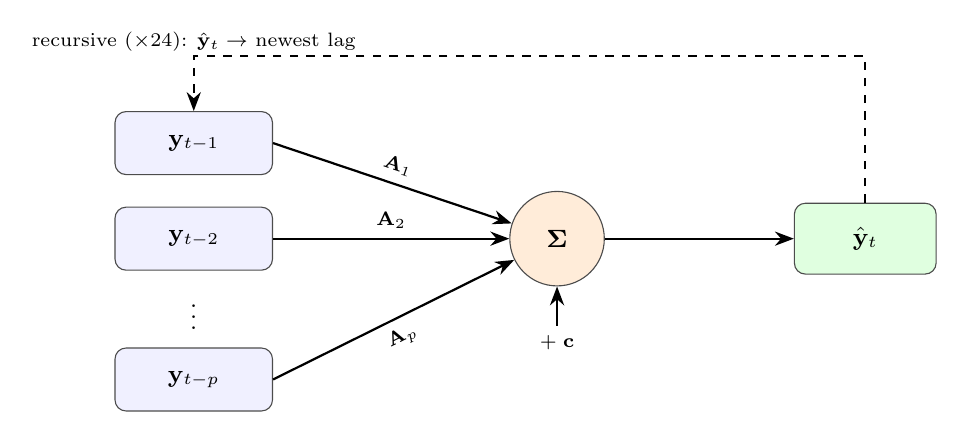
\begin{tikzpicture}[
  every node/.style={font=\small},
  yv/.style={rectangle, rounded corners, draw=black!70, fill=blue!6,
             minimum width=20mm, minimum height=8mm, align=center},
  sum/.style={circle, draw=black!70, fill=orange!15, minimum size=12mm, inner sep=1pt},
  obox/.style={rectangle, rounded corners, draw=black!70, fill=green!12,
              minimum width=18mm, minimum height=9mm, align=center},
  arr/.style={-{Stealth[length=2.4mm]}, thick}
]
\node[yv] (y1) {$\mathbf{y}_{t-1}$};
\node[yv, below=4mm of y1] (y2) {$\mathbf{y}_{t-2}$};
\node[below=1mm of y2] (d) {$\vdots$};
\node[yv, below=1mm of d] (yp) {$\mathbf{y}_{t-p}$};
\node[sum, right=30mm of y2] (S) {$\boldsymbol{\Sigma}$};
\node[obox, right=24mm of S] (yh) {$\hat{\mathbf{y}}_t$};
\node[font=\scriptsize, below=5mm of S] (c) {$+\;\mathbf{c}$};
\draw[arr] (y1.east) -- node[sloped, above, font=\scriptsize] {$\mathbf{A}_1$} (S);
\draw[arr] (y2.east) -- node[above, font=\scriptsize] {$\mathbf{A}_2$} (S);
\draw[arr] (yp.east) -- node[sloped, below, font=\scriptsize] {$\mathbf{A}_p$} (S);
\draw[arr] (c) -- (S);
\draw[arr] (S) -- (yh);
\draw[arr, dashed] (yh.north) |- ([yshift=7mm]y1.north) -- (y1.north);
\node[font=\scriptsize, fill=white, inner sep=1.5pt, above=7mm of y1]
  {recursive ($\times 24$): $\hat{\mathbf{y}}_t \to$ newest lag};
\end{tikzpicture}
\caption{VAR prediction structure. The lagged state vectors
$\mathbf{y}_{t-1},\dots,\mathbf{y}_{t-p}$ (each a $7$-vector of
\texttt{temp,rh,dew,pressure,cloud,wx,wy}) are mapped through the coefficient
matrices $\mathbf{A}_1,\dots,\mathbf{A}_p$ and summed with the intercept $\mathbf{c}$
to give the one-step forecast $\hat{\mathbf{y}}_t$; the prediction is appended as the
newest lag and the window rolled forward, repeated $24$ times for the full horizon.}
\label{fig:var-structure}
\end{figure}

\paragraph{Estimation.}
Because every equation shares the same regressors (the stacked lags), VAR is
estimated by \textbf{equation-by-equation OLS}, which equals the Gaussian maximum-
likelihood estimator. Fitting is therefore closed-form and seed-free.

\paragraph{Lag-order selection.}
The order $p$ minimises the Akaike Information Criterion over
$p\in\{1,\dots,p_{\max}\}$,
\begin{equation}
  \mathrm{AIC}(p) = \ln\big|\hat{\bm{\Sigma}}(p)\big| + \frac{2}{T}\,p\,k^2 ,
  \label{eq:var-aic}
\end{equation}
trading goodness of fit against the $k^2p$ parameters.

\paragraph{Stability and forecast intervals.}
The process is stable (hence stationary) iff every root $z$ of
$\det(\mathbf{I}_k - \mathbf{A}_1 z - \dots - \mathbf{A}_p z^p)=0$ lies outside the
unit circle. Forecasts are produced recursively from Eq.~\eqref{eq:var}; the
$h$-step error covariance is
\begin{equation}
  \bm{\Sigma}(h) = \sum_{j=0}^{h-1} \bm{\Phi}_j \, \bm{\Sigma} \, \bm{\Phi}_j^{\top},
  \label{eq:var-fcse}
\end{equation}
with moving-average matrices $\bm{\Phi}_j$, giving the analytic band
$\hat{y}_v(h) \pm z_{1-\alpha/2}\sqrt{[\bm{\Sigma}(h)]_{vv}}$. Equation
\eqref{eq:var-fcse} assumes Gaussian innovations --- an assumption violated here
(Section~\ref{sec:var-diag}), motivating the bootstrap interval below.

\subsection{Model Specification and Training}
\label{sec:var-train}
\paragraph{Stationarity and differencing order.}
An Augmented Dickey--Fuller (ADF) test on each training series rejects the unit-root
null at $p \le 10^{-8}$ for all seven targets (Table~\ref{tab:var-diag}), so the
model is fit on \emph{levels} ($d=0$). The borderline KPSS results for \texttt{temp}
and \texttt{wx} (Chapter~\ref{ch:eda}) reflect the deterministic \emph{annual} cycle
rather than a stochastic trend, which differencing would not remove.

\paragraph{Lag order.}
Minimising AIC (Eq.~\eqref{eq:var-aic}) over $p_{\max}=60$ selects $\mathbf{p=50}$,
a genuine interior minimum (the criterion rises for $p>50$); the more parsimonious
BIC and HQIC prefer $p=26$. We adopt the AIC choice, which also yields white-noise
residuals (Section~\ref{sec:var-diag}). The model is fit once on the 2021--2023
partition (26{,}280 hourly rows) by OLS; being deterministic, it needs no seed
ensemble (contrast XGBoost, Section~\ref{sec:xgb-train}).

\begin{table}[H]\centering
\caption{VAR configuration.}
\label{tab:var-config}
\begin{tabular}{ll}
\toprule
\textbf{Setting} & \textbf{Value} \\
\midrule
Variables $k$            & 7 (\texttt{temp,rh,dew,pressure,cloud,wx,wy}) \\
Estimation               & equation-by-equation OLS (deterministic) \\
Differencing $d$         & 0 (levels; ADF) \\
Lag search $p_{\max}$    & 60 \\
Selected lag $p$ (AIC)   & 50 \\
Parameters $k(kp{+}1)$   & 2{,}457 \\
Training rows            & 26{,}280 (2021--2023) \\
\bottomrule
\end{tabular}
\end{table}

\subsection{Forecasting Procedure}
\label{sec:var-predict}
The end-to-end VAR pipeline --- from raw hourly data through specification,
estimation, and diagnostics to the rolling forecast --- is summarised in
Figure~\ref{fig:var-pipeline}. At each test origin the last $p$ observed rows seed a
recursive $24$-step forecast (the feedback structure of Fig.~\ref{fig:var-structure}),
which is inverted to the real scale before scoring;
the rolling-origin loop matches the shared protocol
(Section~\ref{sec:eval-protocol}). Algorithm~\ref{alg:var} gives the procedure in
detail.

\begin{figure}[H]
\centering
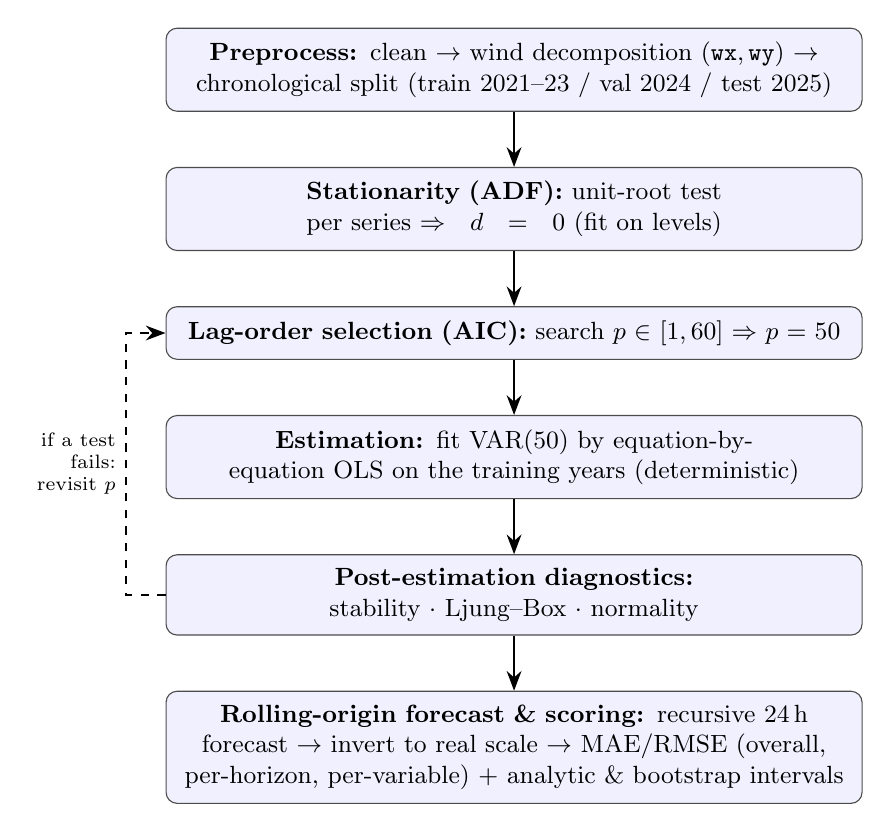
\begin{tikzpicture}[
  node distance=7mm,
  box/.style={rectangle, rounded corners, draw=black!70, fill=blue!6,
              text width=0.70\textwidth, align=center, inner sep=5pt, font=\small},
  arr/.style={-{Stealth[length=2.5mm]}, thick}
]
\node[box] (p1) {\textbf{Preprocess:} clean $\rightarrow$ wind decomposition $(\texttt{wx},\texttt{wy})$ $\rightarrow$ chronological split (train 2021--23 / val 2024 / test 2025)};
\node[box, below=of p1] (p2) {\textbf{Stationarity (ADF):} unit-root test per series $\Rightarrow d=0$ (fit on levels)};
\node[box, below=of p2] (p3) {\textbf{Lag-order selection (AIC):} search $p \in [1,60] \Rightarrow p=50$};
\node[box, below=of p3] (p4) {\textbf{Estimation:} fit $\mathrm{VAR}(50)$ by equation-by-equation OLS on the training years (deterministic)};
\node[box, below=of p4] (p5) {\textbf{Post-estimation diagnostics:} stability $\cdot$ Ljung--Box $\cdot$ normality};
\node[box, below=of p5] (p6) {\textbf{Rolling-origin forecast \& scoring:} recursive 24\,h forecast $\rightarrow$ invert to real scale $\rightarrow$ MAE/RMSE (overall, per-horizon, per-variable) $+$ analytic \& bootstrap intervals};
\draw[arr] (p1) -- (p2);
\draw[arr] (p2) -- (p3);
\draw[arr] (p3) -- (p4);
\draw[arr] (p4) -- (p5);
\draw[arr] (p5) -- (p6);
\draw[arr, dashed] (p5.west) -- ++(-0.5,0) |- (p3.west)
  node[pos=0.25, left, font=\scriptsize, align=right] {if a test\\ fails:\\ revisit $p$};
\end{tikzpicture}
\caption{VAR modelling pipeline: from raw hourly data to the rolling-origin forecast
and its diagnostics. The dashed arrow is the specification-check feedback ---
re-select the lag order if residual autocorrelation remains.}
\label{fig:var-pipeline}
\end{figure}

\begin{algorithm}[H]
\caption{VAR fitting and rolling-origin evaluation}
\label{alg:var}
\begin{algorithmic}[1]
\Require Hourly series; targets $k{=}7$; $p_{\max}{=}60$; horizon $H{=}24$
\State Preprocess: clean, wind decomposition $(\texttt{wx},\texttt{wy})$; chronological split
\State ADF per series on train $\Rightarrow$ all stationary $\Rightarrow d=0$ (levels)
\State Select $p$ by AIC over $[1,p_{\max}]$ $\Rightarrow p=50$
\State Fit VAR($p$) by OLS on 2021--2023 \Comment{deterministic}
\State Diagnostics: stability, Ljung--Box, normality (Sec.~\ref{sec:var-diag})
\For{each test origin $t$ (step $24$\,h)}
  \State Take last $p$ rows; forecast $t{+}1,\dots,t{+}H$ recursively (Eq.~\eqref{eq:var})
  \State Invert to real scale; compare with actuals
\EndFor
\State Aggregate MAE/RMSE overall, per-horizon, per-variable
\State Intervals: analytic (Eq.~\eqref{eq:var-fcse}) + bootstrap (residual resampling)
\end{algorithmic}
\end{algorithm}

\subsection{Post-estimation Diagnostics}
\label{sec:var-diag}
Before trusting the forecasts we verify the assumptions VAR's validity rests on; the
per-variable results are in Table~\ref{tab:var-diag}.
\begin{itemize}
  \item \textbf{Stationarity (ADF).} All seven series reject the unit-root null
        ($p \le 10^{-8}$) $\Rightarrow$ fit on levels ($d=0$).
  \item \textbf{Stability.} Every companion root lies inside the unit circle
        (spectral radius $<1$), so the fitted VAR(50) is stable and its forecasts
        cannot diverge.
  \item \textbf{Residual autocorrelation (Ljung--Box, lag 24).} All seven residual
        series pass ($p>0.05$); \texttt{pressure} is the tightest ($p=0.073$),
        consistent with its longer memory. The residuals are therefore effectively
        white noise --- the chosen lag order leaves no exploitable structure.
  \item \textbf{Normality (Jarque--Bera).} All seven reject normality
        ($p<10^{-3}$), driven by heavy tails (excess kurtosis $6$--$18$) and mild
        skew. This does \emph{not} bias the point forecasts, but it makes the
        \emph{analytic} Gaussian bands of Eq.~\eqref{eq:var-fcse} only approximate;
        we therefore also report a distribution-free \textbf{bootstrap} interval
        that resamples the empirical residuals (Fig.~\ref{fig:var-interval}).
\end{itemize}
In summary, the load-bearing assumptions (stationarity, stability, white-noise
residuals) all hold; only residual normality fails, and only the interval shape ---
not the point forecasts or the error metrics --- depends on it.

\begin{table}[H]\centering
\caption{VAR per-variable diagnostics (residuals of the fitted VAR(50), training set).}
\label{tab:var-diag}
\begin{tabular}{lccccc}
\toprule
\textbf{Variable} & \textbf{ADF $p$} & \textbf{Ljung--Box $p$} & \textbf{Jarque--Bera $p$} & \textbf{Skew} & \textbf{Kurtosis} \\
\midrule
\texttt{temp}     & $1.0\times10^{-8}$  & 0.999 & $<10^{-3}$ & $-1.22$ & 13.74 \\
\texttt{rh}       & $2.8\times10^{-23}$ & 1.000 & $<10^{-3}$ & $ 0.52$ &  8.84 \\
\texttt{dew}      & $7.6\times10^{-10}$ & 1.000 & $<10^{-3}$ & $-0.45$ & 17.82 \\
\texttt{pressure} & $2.1\times10^{-10}$ & 0.073 & $<10^{-3}$ & $ 0.09$ &  5.85 \\
\texttt{cloud}    & $2.8\times10^{-27}$ & 1.000 & $<10^{-3}$ & $-0.13$ &  8.13 \\
\texttt{wx}       & $1.1\times10^{-24}$ & 1.000 & $<10^{-3}$ & $ 0.44$ & 10.26 \\
\texttt{wy}       & $5.5\times10^{-26}$ & 1.000 & $<10^{-3}$ & $ 0.07$ &  8.49 \\
\bottomrule
\end{tabular}
\end{table}
Stability holds globally (spectral radius $<1$) and the joint multivariate normality
test is likewise rejected ($p\approx0$), in line with the per-variable verdicts.

\subsection{Experimental Results}
\label{sec:var-results}
Evaluated by rolling-origin over 2025 ($N=364$ origins, real scale; 95\% CIs from
$1000$ origin bootstraps), VAR(50) attains an \textbf{overall MAE of $5.57$} and
\textbf{RMSE of $12.07$} (Table~\ref{tab:var-overall}); being an OLS fit it is
exactly deterministic, so no seed spread is reported. The per-variable breakdown
(Table~\ref{tab:var-pervar}) mirrors the pattern of every model in this study:
\texttt{temp}, \texttt{dew}, and \texttt{pressure} are forecast tightly
($R^2 \ge 0.92$, MAE $\approx 1.1$ in native units), while \texttt{cloud} is by far
the hardest ($R^2=0.37$, MAE $22.8\%$) --- the bimodal, weakly-correlated target
flagged in the EDA. Error grows smoothly with lead time, from MAE $2.27$ at $h{=}1$
to $6.81$ at $h{=}24$ (Fig.~\ref{fig:var-horizon}), and the forecasts track the
actuals closely for the well-modelled variables (Fig.~\ref{fig:var-pva}). Notably,
this linear, fully interpretable model lands within $\sim$2\% MAE of the much more
complex XGBoost (overall MAE $5.48$, Section~\ref{sec:xgb-results}) and is
essentially tied with the LSTM on per-variable $R^2$ (e.g.\ \texttt{temp}
$0.918$ vs.\ $0.921$; \texttt{pressure} $0.954$ vs.\ $0.941$), while additionally
supplying formal diagnostics and analytic uncertainty bands.

\begin{table}[H]\centering
\caption{VAR --- overall test metrics (real scale, 2025; $N=364$ origins, 95\% bootstrap CI).}
\label{tab:var-overall}
\begin{tabular}{lcc}
\toprule
\textbf{Metric} & \textbf{Value} & \textbf{95\% bootstrap CI} \\
\midrule
Overall MAE  & 5.57  & $[5.38,\ 5.78]$   \\
Overall RMSE & 12.07 & $[11.60,\ 12.57]$ \\
\bottomrule
\end{tabular}
\end{table}

\begin{table}[H]\centering
\caption{VAR --- per-variable error (real scale, horizon-averaged, 2025; $R^2$ vs.\ test mean).}
\label{tab:var-pervar}
\begin{tabular}{lrrrrrrr}
\toprule
 & \texttt{temp} & \texttt{rh} & \texttt{dew} & \texttt{pressure} & \texttt{cloud} & \texttt{wx} & \texttt{wy} \\
 & ($^\circ$C) & (\%) & ($^\circ$C) & (hPa) & (\%) & (km/h) & (km/h) \\
\midrule
MAE   & 1.11 & 5.60 & 1.10 & 1.10 & 22.82 & 4.22 & 3.05 \\
RMSE  & 1.55 & 7.51 & 1.59 & 1.63 & 30.08 & 5.74 & 4.28 \\
$R^2$ & 0.92 & 0.76 & 0.94 & 0.95 & 0.37 & 0.52 & 0.29 \\
\bottomrule
\end{tabular}
\end{table}

\begin{figure}[H]\centering
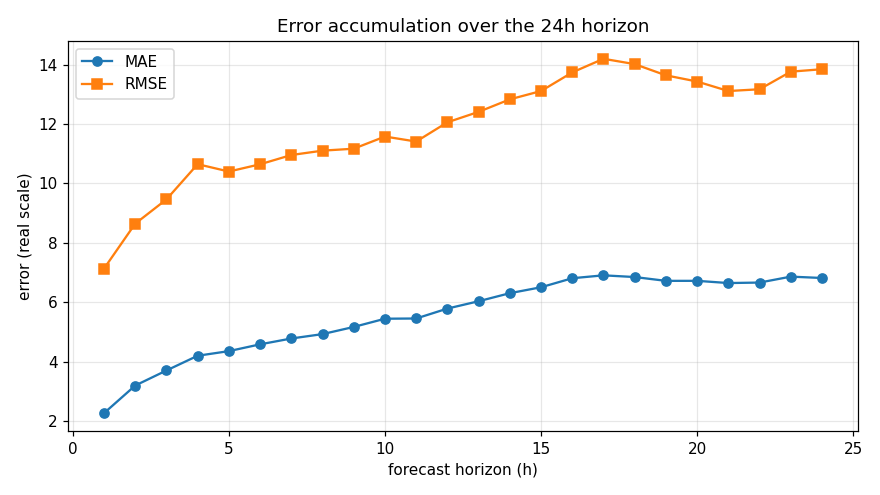
\includegraphics[width=0.8\textwidth]{var_per_horizon.png}
\caption{VAR: error accumulation over the 24-hour horizon (2025 test).}
\label{fig:var-horizon}
\end{figure}

\begin{figure}[H]\centering
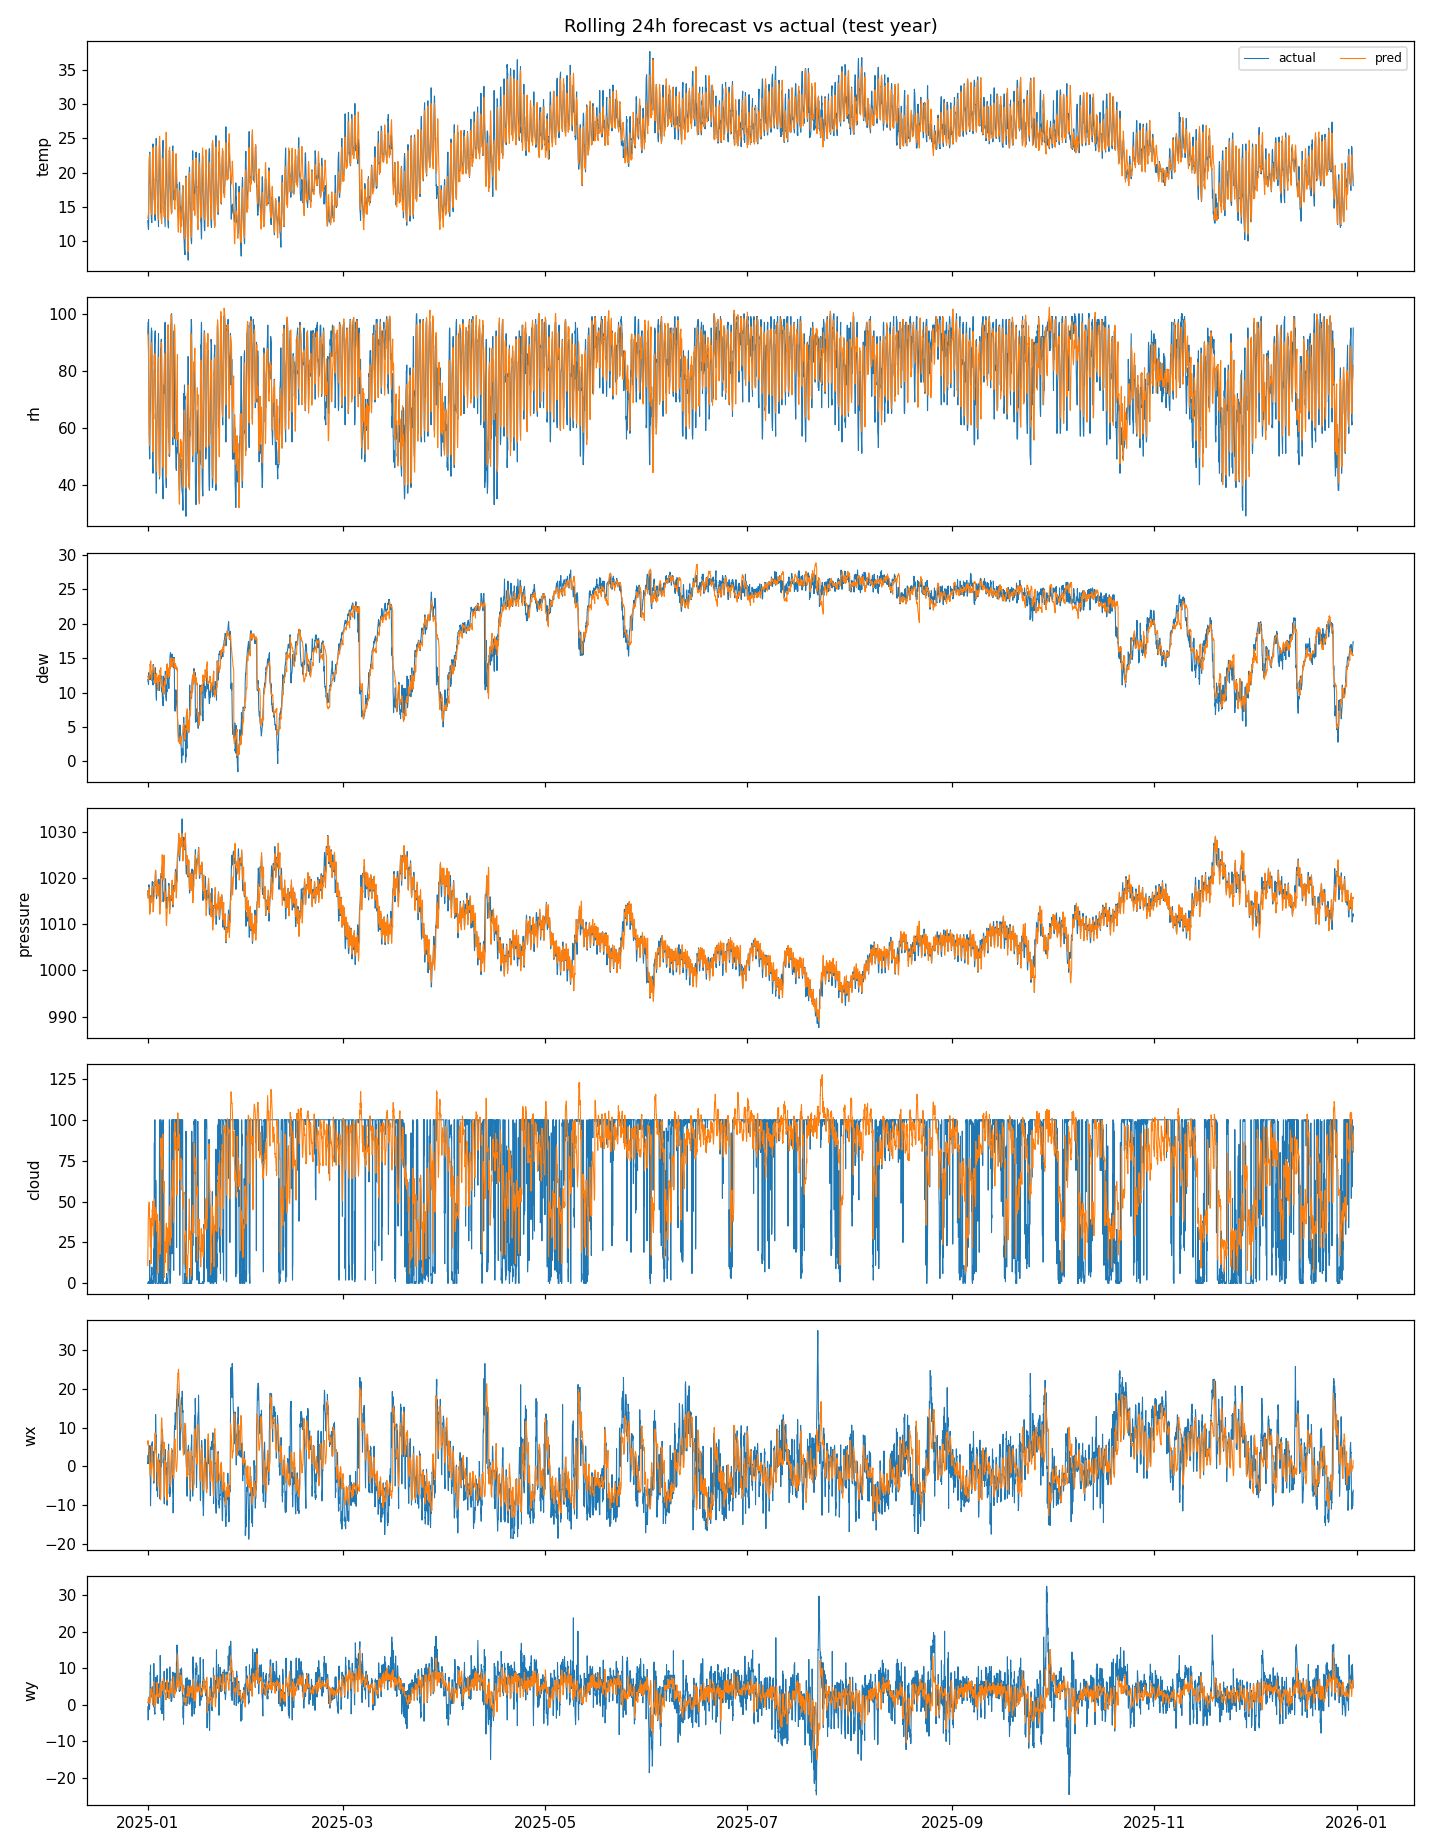
\includegraphics[width=\textwidth]{var_pred_vs_actual.png}
\caption{VAR: rolling 24-hour forecast vs.\ actual across the 2025 test year.}
\label{fig:var-pva}
\end{figure}

\begin{figure}[H]\centering
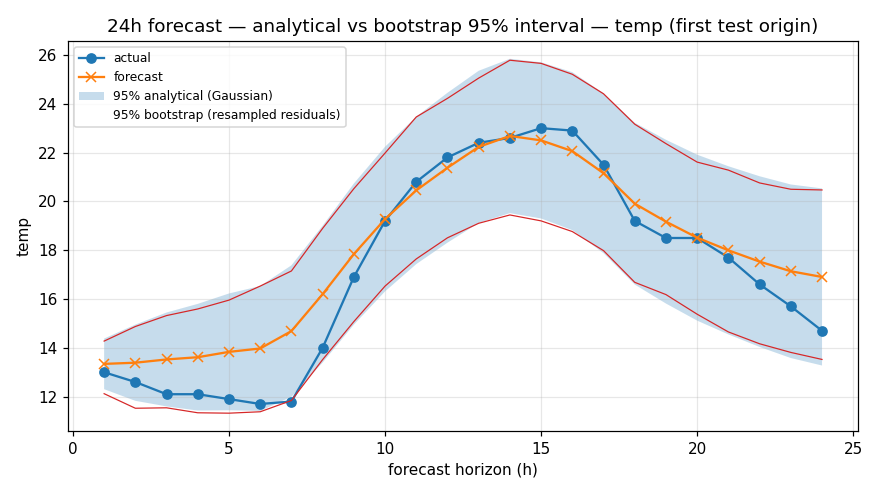
\includegraphics[width=0.8\textwidth]{var_forecast_interval.png}
\caption{VAR: 24-hour \texttt{temp} forecast at the first 2025 origin with 95\%
analytic (Gaussian) and bootstrap (resampled-residual) intervals.}
\label{fig:var-interval}
\end{figure}

%--------------------------------------------------------------- XGBOOST (detailed)
\section{XGBoost}
\label{sec:xgboost}

\subsection{Overview}
\label{sec:xgb-overview}
XGBoost is a scalable gradient-boosted decision-tree system \citep{chen2016xgboost}.
In this project the $24$-hour-ahead multivariate forecast is produced by
\textbf{seven multi-output regressors}, one per target variable; each regressor
maps the engineered window features to that variable's $24$ horizon values. This
\emph{direct} (non-recursive) multi-horizon strategy predicts all $24$ lead times
at once and so avoids the error compounding of recursive one-step feedback.

\subsection{Mathematical Formulation}
\label{sec:xgb-theory}
Gradient boosting builds an additive model of $K$ trees,
\[
  \hat{y}_i = \sum_{k=1}^{K} f_k(\mathbf{x}_i), \qquad f_k \in \mathcal{F},
\]
where $\mathcal{F}$ is the space of regression trees. The regularised objective is
\begin{equation}
  \mathcal{L} = \sum_{i} \ell(y_i, \hat{y}_i) + \sum_{k} \Omega(f_k),
  \qquad
  \Omega(f) = \gamma T + \tfrac{1}{2}\lambda \lVert \mathbf{w} \rVert^2,
  \label{eq:xgb-obj}
\end{equation}
with $T$ leaves and leaf weights $\mathbf{w}$. At round $t$, a second-order Taylor
expansion of $\ell$ around the current prediction gives
\begin{equation}
  \mathcal{L}^{(t)} \simeq
  \sum_{i} \Big[ g_i f_t(\mathbf{x}_i) + \tfrac{1}{2} h_i f_t(\mathbf{x}_i)^2 \Big]
  + \Omega(f_t),
  \label{eq:xgb-taylor}
\end{equation}
with first- and second-order gradients
\begin{equation}
  g_i = \partial_{\hat{y}^{(t-1)}} \ell\big(y_i, \hat{y}_i^{(t-1)}\big),
  \qquad
  h_i = \partial^2_{\hat{y}^{(t-1)}} \ell\big(y_i, \hat{y}_i^{(t-1)}\big).
  \label{eq:xgb-grads}
\end{equation}
For a fixed structure with leaf instance sets $I_j$, the optimal leaf weight and
structure score are
\begin{equation}
  w_j^{\star} = -\frac{\sum_{i \in I_j} g_i}{\sum_{i \in I_j} h_i + \lambda},
  \qquad
  \tilde{\mathcal{L}} = -\tfrac{1}{2}\sum_{j=1}^{T}
  \frac{\big(\sum_{i \in I_j} g_i\big)^2}{\sum_{i \in I_j} h_i + \lambda}
  + \gamma T ,
  \label{eq:xgb-leaf}
\end{equation}
and splits are chosen greedily to maximise the gain implied by
Eq.~\eqref{eq:xgb-leaf}. With the squared-error loss
$\ell = \tfrac{1}{2}(y_i-\hat{y}_i)^2$ used here, $g_i = \hat{y}_i - y_i$ and
$h_i = 1$.

\subsection{Feature Engineering}
\label{sec:xgb-fe}
A decision tree splits on individual tabular features and cannot exploit a raw,
flattened $120 \times d_{\text{in}}$ window --- each of the $\sim$1.3k cells would
be a near-duplicate column with little standalone signal. The window is therefore
\emph{summarised} into compact per-channel descriptors that expose the level,
recent change, volatility, and range of each channel to the splitting criterion.
With $7$ weather channels the construction yields
$7 \times 20 + 4 = \mathbf{144}$ features. Crucially, \emph{every} feature uses
only history up to the origin $e$ (lags use $e-L$; rolling statistics use the
window $[e-w+1,\,e]$), so it shares the exact no-leakage horizon of the raw window.
In practice the rolling operators are computed once over the whole series and then
sampled at the origins, which is both fast and leakage-safe.

\subsubsection{Lag Features}
For channel $c$ and lag set $\mathcal{S}_{\text{lag}} = \{0,1,2,3,6,12,24,48,72,119\}$,
\[
  \text{lag}^{(c)}_{L}(e) = x^{(c)}_{e-L}, \qquad L \in \mathcal{S}_{\text{lag}}.
\]
The short lags ($0$--$6$\,h) capture the immediate trajectory, $12$/$24$\,h capture
the diurnal cycle, and $48$--$119$\,h capture multi-day persistence.

\subsubsection{Rolling Mean Features}
For windows $w \in \{3,6,12,24,72\}$,
\[
  \text{mean}^{(c)}_{w}(e) = \frac{1}{w}\sum_{i=0}^{w-1} x^{(c)}_{e-i},
\]
smoothing the channel at intra-day to multi-day scales to give the tree a denoised
level signal.

\subsubsection{Rolling Standard-Deviation Features}
For windows $w \in \{6,24,120\}$,
\[
  \text{std}^{(c)}_{w}(e) =
  \sqrt{\frac{1}{w-1}\sum_{i=0}^{w-1}\big(x^{(c)}_{e-i} - \text{mean}^{(c)}_{w}(e)\big)^2},
\]
summarising short- and long-range volatility (how unsettled recent weather has
been), which lets the model sharpen or widen its response.

\subsubsection{Rolling Min/Max (Range) Features}
A $24$-hour minimum and maximum per weather channel describe the recent daily
range,
\[
  \text{min}^{(c)}_{24}(e) = \min_{0 \le i < 24} x^{(c)}_{e-i},
  \qquad
  \text{max}^{(c)}_{24}(e) = \max_{0 \le i < 24} x^{(c)}_{e-i}.
\]

\subsubsection{Time-based Features}
The four cyclical encodings $(\text{hour}_{\sin}, \text{hour}_{\cos},
\text{doy}_{\sin}, \text{doy}_{\cos})$ are taken at the origin so the model knows
``what time it is now''. The EDA (Chapter~\ref{ch:eda}) showed strong diurnal and
annual cycles, which these encodings make directly available to the trees.

\subsection{Training Procedure}
\label{sec:xgb-train}
\paragraph{One regressor per target.}
Seven independent regressors are trained, one per target; each predicts that
variable's $24$ horizons simultaneously using the default
\texttt{one\_output\_per\_tree} multi-output strategy. The vector-leaf
\texttt{multi\_output\_tree} mode was tested and rejected --- on this feature set
it was roughly an order of magnitude slower for no accuracy gain.

\paragraph{Data usage and windows.}
Models are fit on the 2021--2023 training windows with a $6$-hour origin step:
consecutive hourly windows are near-identical, so a $6$-hour step retains
$\sim$4.4k diverse windows at a fraction of the cost, with negligible accuracy
loss. The $24$-hour evaluation step is unaffected.

\paragraph{Validation and early stopping.}
The number of boosting rounds is the \emph{only} quantity chosen from data:
training monitors the 2024 validation RMSE and stops when it has not improved for
$25$ rounds (cap $400$). All other hyperparameters (Table~\ref{tab:xgb-hparams})
are fixed \emph{a priori} --- there is no grid search --- and the 2025 test set is
never seen during training.

\paragraph{Determinism.}
Because subsampling makes the learner stochastic, three seeds $\{0,1,2\}$ are
trained and reported as a seed ensemble together with the per-seed standard
deviation.

\begin{table}[H]
\centering
\caption{XGBoost hyperparameters (fixed a priori; trees chosen by early stopping).}
\label{tab:xgb-hparams}
\begin{tabular}{ll}
\toprule
\textbf{Parameter} & \textbf{Value} \\
\midrule
objective             & \texttt{reg:squarederror} \\
tree method           & \texttt{hist} \\
n\_estimators (cap)   & 400 \\
early stopping rounds & 25 \\
learning rate         & 0.08 \\
max depth             & 6 \\
subsample             & 0.8 \\
colsample\_bytree     & 0.6 \\
min\_child\_weight    & 5.0 \\
reg\_lambda           & 1.0 \\
train origin step     & 6\,h \\
seeds                 & \{0, 1, 2\} \\
\bottomrule
\end{tabular}
\end{table}

\subsection{Prediction Pipeline}
\label{sec:xgb-predict}
\begin{enumerate}
  \item \textbf{Preprocessing:} clean, decompose wind, add time encodings, and
        scale with the train-fit \texttt{StandardScaler}.
  \item \textbf{Feature generation:} encode the $120$-hour window ending at the
        origin into the $144$ features of Section~\ref{sec:xgb-fe}.
  \item \textbf{Prediction:} each regressor outputs its $24$ scaled horizon values;
        stacking the seven gives a $24 \times 7$ block (averaged over seeds).
  \item \textbf{Post-processing:} invert the scaler to the real scale before
        scoring; optional empirical residual intervals quantify uncertainty.
\end{enumerate}

\subsection{Algorithm}
\label{sec:xgb-algo}
\begin{algorithm}[H]
\caption{XGBoost direct multi-horizon forecasting (training + rolling evaluation)}
\label{alg:xgb}
\begin{algorithmic}[1]
\Require Hourly series; lookback $L=120$; horizon $H=24$; targets $V=7$; seeds
\State Preprocess: clean, wind decomposition, time encodings
\State Fit \texttt{StandardScaler} on train; transform all splits
\State Build engineered windows $(\mathbf{X}, \mathbf{Y})$ for train/val/test
\For{each seed}
  \For{each target variable $v \in \{1,\dots,V\}$}
    \State Train multi-output XGBoost $\mathbf{X}_{\text{tr}} \!\to\! \mathbf{Y}_{\text{tr}}[:,:,v]$
    \State Early-stop on $(\mathbf{X}_{\text{val}}, \mathbf{Y}_{\text{val}}[:,:,v])$
  \EndFor
\EndFor
\For{each test origin $t$ (step $24$ h)} \Comment{rolling-origin evaluation}
  \State Encode window ending at $t$; predict $\hat{\mathbf{Y}} \in \mathbb{R}^{H\times V}$
  \State Inverse-transform $\hat{\mathbf{Y}}$ to real scale; compare to actuals
\EndFor
\State Aggregate MAE/RMSE overall, per-horizon, per-variable; bootstrap CIs
\end{algorithmic}
\end{algorithm}

\subsection{Experimental Results}
\label{sec:xgb-results}
Evaluated by rolling-origin over the 2025 test year ($N=365$ origins, real scale),
the seed-ensemble XGBoost attains an \textbf{overall MAE of $5.48$} (95\% bootstrap
CI $[5.28, 5.69]$) and \textbf{RMSE of $11.93$} ($[11.44, 12.40]$); the seed
standard deviation is only $0.016$ (MAE), i.e.\ the model is effectively
deterministic (Table~\ref{tab:xgb-overall}). The overall figure mixes units, so the
per-variable breakdown (Table~\ref{tab:xgb-pervar}) is more informative:
temperature, dew point, and pressure are forecast tightly (MAE $\approx 1$ in their
native units), whereas \texttt{cloud} is by far the hardest (MAE $22.4\%$) ---
consistent with its weak correlations and bimodal distribution seen in the EDA
(Chapter~\ref{ch:eda}). Error grows smoothly with lead time, from MAE $2.26$ at
$h{=}1$ to $6.79$ at $h{=}24$ before plateauing (Fig.~\ref{fig:xgb-horizon}); the
validation learning curves converge without divergence
(Fig.~\ref{fig:xgb-learn}); and the forecasts track the actuals closely for the
well-modelled variables (Fig.~\ref{fig:xgb-pva}).

\begin{table}[H]\centering
\caption{XGBoost --- overall test metrics (real scale, 2025; seed ensemble $\{0,1,2\}$).}
\label{tab:xgb-overall}
\begin{tabular}{lrcr}
\toprule
\textbf{Metric} & \textbf{Value} & \textbf{95\% bootstrap CI} & \textbf{seed std} \\
\midrule
Overall MAE  & 5.48  & $[5.28,\ 5.69]$   & 0.016 \\
Overall RMSE & 11.93 & $[11.44,\ 12.40]$ & 0.012 \\
\bottomrule
\end{tabular}
\end{table}

\begin{table}[H]\centering
\caption{XGBoost --- per-variable error (real scale, horizon-averaged, 2025).}
\label{tab:xgb-pervar}
\begin{tabular}{lrrrrrrr}
\toprule
 & \texttt{temp} & \texttt{rh} & \texttt{dew} & \texttt{pressure} & \texttt{cloud} & \texttt{wx} & \texttt{wy} \\
 & ($^\circ$C) & (\%) & ($^\circ$C) & (hPa) & (\%) & (km/h) & (km/h) \\
\midrule
MAE  & 1.06 & 5.43 & 1.08 & 1.24 & 22.42 & 4.15 & 2.99 \\
RMSE & 1.49 & 7.45 & 1.63 & 1.80 & 29.73 & 5.67 & 4.17 \\
\bottomrule
\end{tabular}
\end{table}

\begin{figure}[H]\centering
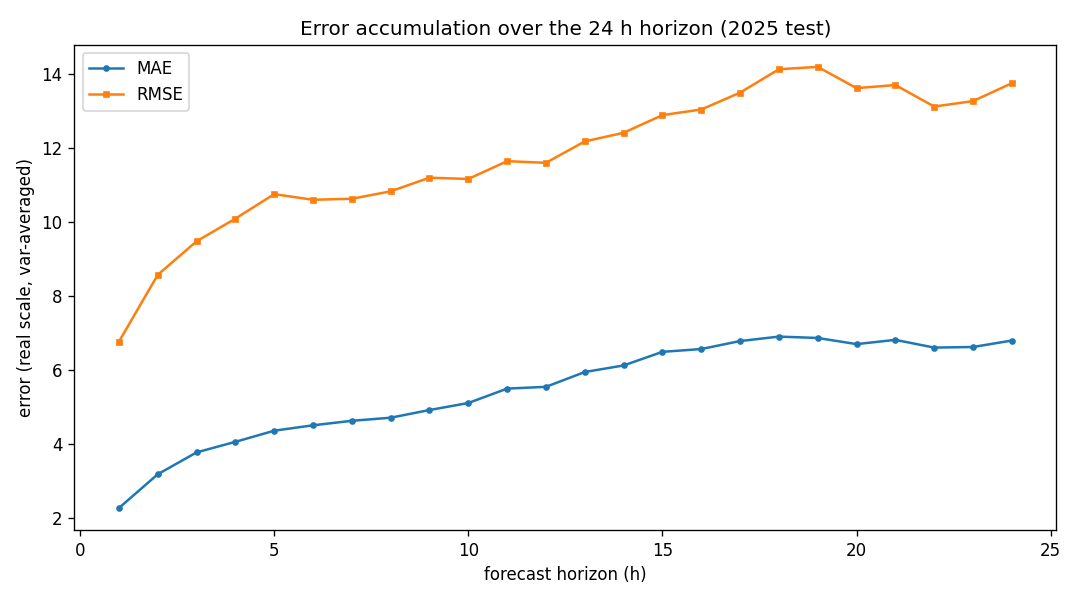
\includegraphics[width=0.8\textwidth]{xgb_per_horizon.png}
\caption{XGBoost: error accumulation over the 24-hour horizon (2025 test).}
\label{fig:xgb-horizon}
\end{figure}

\begin{figure}[H]\centering
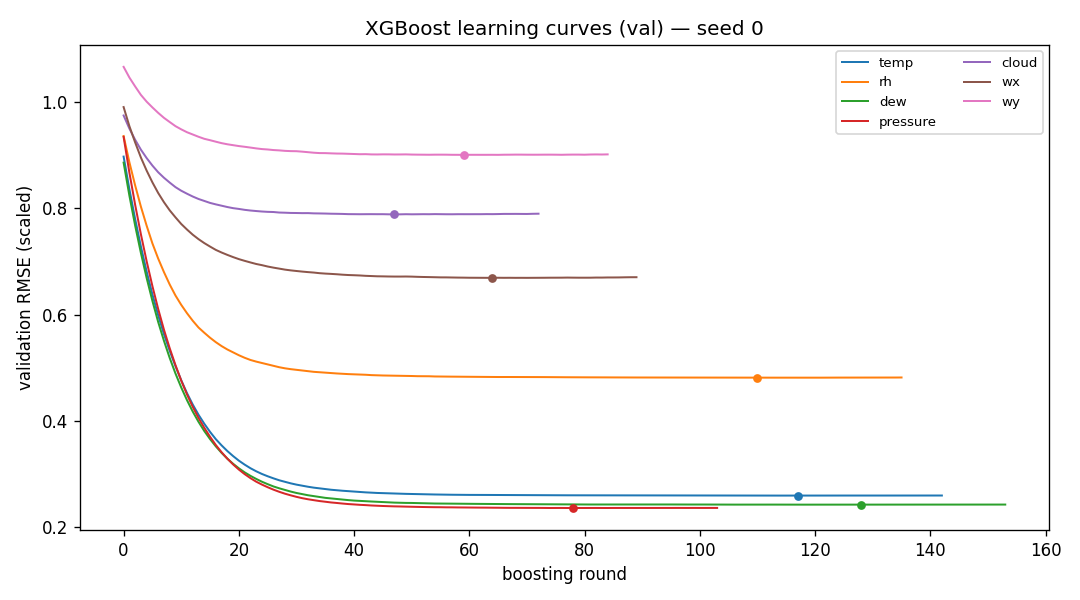
\includegraphics[width=0.78\textwidth]{xgb_learning_curves.png}
\caption{XGBoost: validation-RMSE learning curves (seed 0), one curve per target.}
\label{fig:xgb-learn}
\end{figure}

\begin{figure}[H]\centering
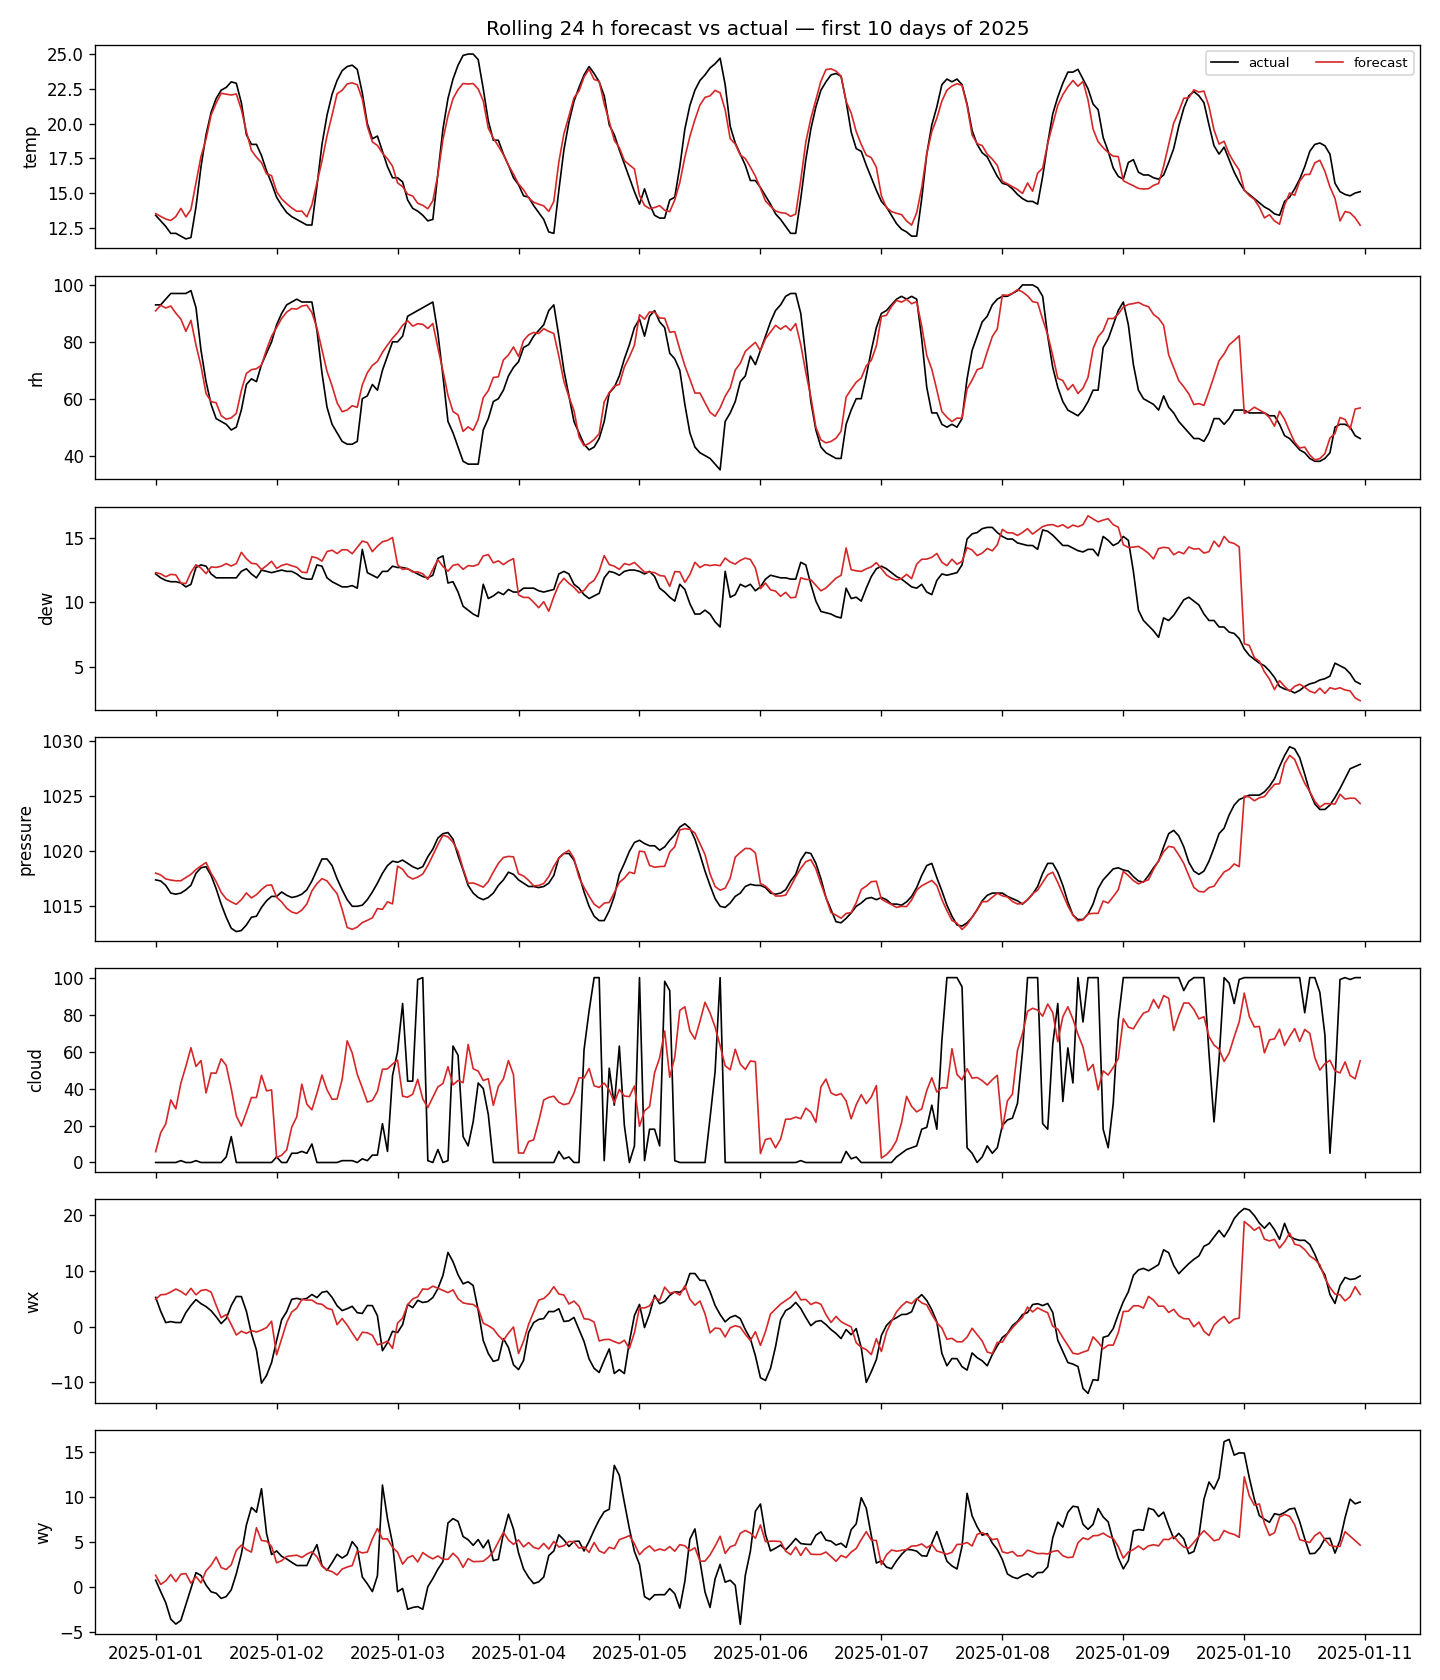
\includegraphics[width=\textwidth]{xgb_pred_vs_actual.png}
\caption{XGBoost: rolling 24-hour forecast vs.\ actual, first 10 days of 2025.}
\label{fig:xgb-pva}
\end{figure}

%--------------------------------------------------------------- LSTM
\section{LSTM}
\label{sec:lstm}
\subsection{Overview}
The Long Short-Term Memory network is a recurrent architecture that learns
long-range temporal dependencies via gated memory cells \citep{hochreiter1997lstm}.
An encoder LSTM consumes the $120$-hour input window and its final hidden state is
mapped (directly or through a decoder) to the $24 \times 7$ forecast block. It
models nonlinear temporal dependencies without hand-crafted lags, but is more data-
and compute-hungry, sensitive to hyperparameters, and less interpretable than the
other models.

\subsection{Mathematical Formulation}
At each temporal step $t \in [1, 120]$, the LSTM cell processes the input vector $x_t \in \mathbb{R}^{12 \times 1}$ and the previous hidden state $h_{t-1} \in \mathbb{R}^{128 \times 1}$ (given 128 hidden units). To optimize GPU-accelerated tensor computations, the hidden state and input vector are concatenated into a unified vector $[h_{t-1}, x_t] \in \mathbb{R}^{140 \times 1}$. 

The internal mechanics are governed by four primary equations that compute the activations of the forget gate ($f_t$), input gate ($i_t$), candidate cell state ($\tilde{c}_t$), and output gate ($o_t$):

\begin{align}
f_t &= \sigma(W_f [h_{t-1}, x_t] + b_f) \label{eq:lstm_forget} \\
i_t &= \sigma(W_i [h_{t-1}, x_t] + b_i) \label{eq:lstm_input} \\
\tilde{c}_t &= \tanh(W_c [h_{t-1}, x_t] + b_c) \label{eq:lstm_candidate} \\
o_t &= \sigma(W_o [h_{t-1}, x_t] + b_o) \label{eq:lstm_output}
\end{align}

where:
\begin{itemize}
    \item $W_f, W_i, W_c, W_o \in \mathbb{R}^{128 \times 140}$ represent the learnable weight matrices (equivalent to the partitioned matrices $W_{xh} \in \mathbb{R}^{128 \times 12}$ and $W_{hh} \in \mathbb{R}^{128 \times 128}$). These matrices act as static, learned filters that remain constant during inference.
    \item $b_f, b_i, b_c, b_o \in \mathbb{R}^{128 \times 1}$ are the learnable bias vectors.
    \item $\sigma(z) = \frac{1}{1 + e^{-z}}$ is the logistic sigmoid function, mapping any real input strictly to the range $(0, 1)$ to serve as scaling coefficients.
    \item $\tanh(z) = \frac{e^z - e^{-z}}{e^z + e^{-z}}$ is the hyperbolic tangent function, mapping values to the range $(-1, 1)$ to establish zero-centered candidate signals.
\end{itemize}

Once the gates are computed, the cell state $c_t \in \mathbb{R}^{128 \times 1}$ (carrying long-term sequence trends and contextual variations across the 120-hour window) and the hidden state $h_t \in \mathbb{R}^{128 \times 1}$ (representing localized working memory and imminent hourly dynamics) are updated via:

\begin{align}
c_t &= f_t \odot c_{t-1} + i_t \odot \tilde{c}_t \label{eq:lstm_cell_update} \\
h_t &= o_t \odot \tanh(c_t) \label{eq:lstm_hidden_update}
\end{align}

Here, $\odot$ denotes the Hadamard (element-wise) product. Rather than acting as stochastic filters, the gating outputs represent precise, deterministic scaling coefficients determined by the inputs and the learned weights.

    \textbf{Dual-Dense Layer Pipeline:} The network directs the final hidden state summary $h_{120}$ through two distinct fully connected (Dense) layers:
    \begin{align}
    h_{dense} &= \text{ReLU}(W_{d1} h_{120} + b_{d1}) \label{eq:dense_1} \\
    \hat{y}_{flat} &= W_{d2} h_{dense} + b_{d2} \label{eq:dense_2}
    \end{align}
    \begin{itemize}
        \item \textit{Dense Layer 1 (Hidden Layer with ReLU):} The Rectified Linear Unit ($\text{ReLU}(z) = \max(0, z)$) is utilized to introduce non-linearity. By clipping negative activations to zero, ReLU encourages sparse representations—allowing specific neurons to specialize in distinct meteorological features—while ensuring robust gradient propagation (preventing vanishing gradients since the gradient of ReLU for positive inputs is a constant $1$).
        \item \textit{Dense Layer 2 (Output Layer with Linear Activation):} To ensure the model can forecast physical values below and above the mean, negative values must not be clipped. Hence, this final layer uses a linear activation function. Because $W_{d2}$ is mathematically unbounded, it acts as a learned linear amplifier, magnifying the signals from the previous layers to project them accurately into any extreme range.
    \end{itemize}

\subsection{Architecture and Regularization}
Unlike tree-based models that require manual feature extraction (e.g., rolling statistics), the LSTM directly digests the raw flattened $120 \times 12$ tensor. The network architecture consists of:
\begin{enumerate}
    \item \textbf{LSTM Layer:} Processes the temporal sequence. The parameter \texttt{return\_sequences=False} ensures only the final hidden state is passed forward.
    \item \textbf{Dropout Layer:} Randomly zeroes out a fraction of connections during training to break co-adaptation among neurons, heavily penalizing overfitting.
    \item \textbf{Hidden Dense Layer:} Uses a Rectified Linear Unit (ReLU) activation to learn non-linear combinations of the LSTM's extracted features.
    \item \textbf{Output Dense \& Reshape:} A linear layer producing exactly $24 \times 7 = 168$ nodes, formatted to match the required protocol output.
\end{enumerate}

\subsection{Training Procedure and Hyperparameter Tuning}
\textbf{Hyperparameter Search Space Strategy:}
Neural networks are highly sensitive to architectural configurations. To prevent data leakage, a systematic grid search is executed strictly on the 2024 validation set. The search space is carefully bounded to balance model capacity and computational efficiency:
\begin{itemize}
    \item \textit{LSTM Units $\{64, 128\}$:} Controls the representational capacity of the network. While 128 units capture more complex meteorological non-linearities, 64 units act as a structural regularizer against overfitting.
    \item \textit{Dropout Rate $\{0.1, 0.2\}$:} Determines the noise injected during training to mitigate neuronal co-adaptation.
    \item \textit{Batch Size $\{64, 128\}$:} A smaller batch provides a noisier, more frequent gradient update to escape local minima, whereas a larger batch stabilizes the gradient descent trajectory.
    \item \textit{Initial Learning Rate $\{10^{-3}, 5 \times 10^{-4}\}$:} Establishes the momentum of the Adam optimizer during the initial epochs.
\end{itemize}

\textbf{Adaptive Optimization (ReduceLROnPlateau):}
Employing a static learning rate often leads to optimization plateaus or divergent oscillations (overshooting) near the global minimum. To address this, an adaptive learning rate schedule is implemented. The network continuously monitors the validation loss (\texttt{val\_loss}). If no improvement is observed for 2 consecutive epochs (a patience threshold), the learning rate is scaled down by a factor of 0.5. This dynamic decay allows the model to take aggressive steps initially and fine-tune its weights meticulously as it approaches the optimal solution.

\textbf{Overfitting Prevention (Early Stopping):}
Coupled with the adaptive learning rate, an Early Stopping mechanism operates with a higher patience of 5 epochs. This hierarchical callback structure ensures that the model is first given opportunities to recover via learning rate reductions. If stagnation persists globally, training halts exactly when the model's generalization capability peaks, automatically restoring the optimal weights and preventing the memorization of training noise.

\textbf{Determinism via Seed Ensemble:} Weight initialization in deep learning is stochastic. To ensure reproducibility and robust reporting as required by the protocol, the final chosen architecture is trained across three fixed random seeds ($42, 123, 2026$). The ultimate forecast is the ensemble mean of these three runs.

\begin{table}[H]
\centering
\caption{LSTM Hyperparameter Configuration and Tuning Details.}
\label{tab:lstm_hyperparams}
\begin{tabular}{ll}
\toprule
\textbf{Hyperparameter / Setting} & \textbf{Value} \\
\midrule
\textit{Architecture \& Data Pipeline} & \\
Lookback Window ($L$) & 120 hours \\
Forecast Horizon ($H$) & 24 hours \\
LSTM Hidden Units & 128 \\
Dropout Rate & 0.1 \\
\midrule
\textit{Optimization} & \\
Optimizer & Adam \\
Initial Learning Rate & 0.001 \\
Batch Size & 64 \\
Loss Function & Mean Squared Error (MSE) \\
\midrule
\textit{Callbacks \& Ensemble} & \\
ReduceLROnPlateau Factor & 0.5 (Patience: 4 epochs) \\
Early Stopping Patience & 12 epochs \\
Ensemble Random Seeds & 42, 123, 2026 \\
\bottomrule
\end{tabular}
\end{table}

\subsection{Algorithm}

\begin{algorithm}[H]
\caption{LSTM Direct Multi-horizon Forecasting (Tuning \& Evaluation)}
\label{alg:lstm}
\begin{algorithmic}[1]
\Require Hourly series; lookback $L=120$; horizon $H=24$; targets $V=7$; seeds $S=\{42, 123, 2026\}$
\State Preprocess: clean, decompose wind, encode time, scale via StandardScaler
\State Generate sliding windows $(X, Y)$ for train (2021-2023), val (2024), test (2025)
\State \textbf{Phase 1: Hyperparameter Tuning}
\For{each combination of (units, dropout, batch\_size, learning\_rate)}
    \State Initialize Adam optimizer with \textit{learning\_rate}
    \State Train model on $X_{tr}, Y_{tr}$, monitor $MSE$ on $X_{val}, Y_{val}$
    \State Apply \textit{ReduceLROnPlateau} (patience=2, factor=0.5)
    \State Apply \textit{EarlyStopping} (patience=3)
\EndFor
\State Select best hyperparameters $P_{best}$ based on minimum $val\_loss$
\State \textbf{Phase 2: Ensemble Training \& Evaluation}
\For{each seed $s \in S$}
    \State Set global random seed $s$
    \State Initialize LSTM with $P_{best}$
    \State Train on $X_{tr}, Y_{tr}$, early-stop on $X_{val}, Y_{val}$ (patience=5)
    \State Predict $\hat{Y}_{scaled}^{(s)}$ on $X_{test}$
    \State Inverse transform $\hat{Y}_{scaled}^{(s)} \rightarrow \hat{Y}_{real}^{(s)}$
\EndFor
\State Calculate Ensemble Mean: $\hat{Y}_{ens} = \frac{1}{|S|} \sum \hat{Y}_{real}^{(s)}$
\State Compute MAE, RMSE (overall, per-horizon, per-variable) on $\hat{Y}_{ens}$ vs $Y_{test}$
\end{algorithmic}
\end{algorithm}

\subsection{Post-estimation Diagnostics}
Post-estimation diagnostics were conducted on the $h=1$ forecast residuals to validate the model specification. The Ljung-Box test (evaluated at lag 24) assesses whether the residuals resemble independent white noise. 

The LSTM successfully captured the underlying dynamics for \texttt{rh} ($p=0.0608$), \texttt{cloud} ($p=0.2695$), \texttt{wx} ($p=0.3948$), and \texttt{wy} ($p=0.1264$), all yielding $p > 0.05$ (Pass). This is a significant achievement, demonstrating that the LSTM effectively extracted all structural patterns from highly chaotic variables like wind vectors and cloud cover. 

Conversely, variables characterized by high thermodynamic inertia—such as \texttt{temp} ($p=0.0032$), \texttt{dew} ($p < 0.0001$), and \texttt{pressure} ($p < 0.0001$)—exhibited residual autocorrelation (Fail). This is physically expected: while the model captures macro-level diurnal cycles accurately, micro-level deviations (due to thermal inertia) tend to persist across consecutive hours, causing the residuals to fail the strict independence assumption without degrading the absolute accuracy.

\begin{table}[H]
\centering
\caption{Ljung-Box Residual Diagnostic Results}
\begin{tabular}{lccl}
\toprule
\textbf{Variable} & \textbf{p-value} & \textbf{Result} & \textbf{Status} \\
\midrule
temp     & 0.0032 & Reject $H_0$ & Autocorrelated \\
rh       & 0.0608 & Fail to Reject $H_0$ & White Noise \\
dew      & 0.0000 & Reject $H_0$ & Autocorrelated \\
pressure & 0.0000 & Reject $H_0$ & Autocorrelated \\
cloud    & 0.2695 & Fail to Reject $H_0$ & White Noise \\
wx       & 0.3948 & Fail to Reject $H_0$ & White Noise \\
wy       & 0.1264 & Fail to Reject $H_0$ & White Noise \\
\bottomrule
\end{tabular}
\end{table}

\subsection{Experimental Results}
Evaluated via the rolling-origin method over the 2025 test set, the tuned LSTM Adaptive LR ensemble demonstrates outstanding predictive capability. Table \ref{tab:lstm_overall_metrics} summarizes the overall performance, computed with 1000-iteration Bootstrap 95\% Confidence Intervals.

\begin{table}[H]
\centering
\caption{LSTM Overall Test Metrics (Real Scale, 2025; Ensemble Mean).}
\label{tab:lstm_overall_metrics}
\begin{tabular}{lc}
\toprule
Metric & Value [95\% CI] \\
\midrule
Overall MAE & $5.387 \ [5.157, 5.604]$ \\
Overall RMSE & $12.010 \ [11.435, 12.543]$ \\
Overall $R^2$ Score & $0.9988$ \\
\bottomrule
\end{tabular}
\end{table}

\begin{table}[H]
\centering
\caption{Per-Variable Metrics with Bootstrap 95\% CI on MAE and RMSE.}
\label{tab:lstm_per_var}
\begin{tabular}{lccc}
\toprule
\textbf{Variable} & \textbf{MAE} & \textbf{RMSE} & \textbf{$R^2$ Score} \\
\midrule
Temperature (\texttt{temp}) & $1.109 \ [1.051, 1.173]$ & $1.515 \ [1.416, 1.623]$ & $0.9207$ \\
Relative Humidity (\texttt{rh}) & $5.649 \ [5.359, 5.924]$ & $7.580 \ [7.164, 7.990]$ & $0.7519$ \\
Dew Point (\texttt{dew}) & $1.062 \ [0.982, 1.143]$ & $1.551 \ [1.399, 1.706]$ & $0.9390$ \\
Pressure (\texttt{pressure}) & $1.334 \ [1.244, 1.430]$ & $1.832 \ [1.677, 1.963]$ & $0.9411$ \\
Cloud Cover (\texttt{cloud}) & $21.415 \ [19.961, 22.800]$ & $29.918 \ [28.386, 31.403]$ & $0.3539$ \\
Wind Vector X (\texttt{wx}) & $4.181 \ [3.942, 4.413]$ & $5.668 \ [5.256, 6.048]$ & $0.5352$ \\
Wind Vector Y (\texttt{wy}) & $2.959 \ [2.787, 3.143]$ & $4.116 \ [3.802, 4.459]$ & $0.3452$ \\
\bottomrule
\end{tabular}
\end{table}

\textbf{Variable-Level \& Horizon Analysis:} As detailed in Table \ref{tab:lstm_per_var}, the model achieves an exceptionally high $R^2$ score ($> 0.92$) for core thermodynamic variables (\texttt{temp}, \texttt{dew}, \texttt{pressure}), indicating that the LSTM deeply understands diurnal temperature cycles. Figure \ref{fig:lstm_horizon} maps the error trajectory over the 24-hour future window, demonstrating that the error accumulation is stable and does not exponentially compound, proving the efficacy of the Direct Multi-step architecture. Figure \ref{fig:lstm_actual_pred} visually confirms the network's ability to smoothly trace real-world meteorological fluctuations without outputting flat averages.

\begin{figure}[H]
  \centering
  \framebox{\parbox{0.8\textwidth}{\centering
    \vspace{3cm}
    \textbf{Image Placeholder} \\
    \small\textit{plot\_1\_horizon\_error.png}
    \vspace{3cm}
  }}
  \caption{LSTM: Error accumulation over the 24-hour horizon (Ensemble Mean, 2025 test).}
  \label{fig:lstm_horizon}
\end{figure}

\begin{figure}[H]
  \centering
  \framebox{\parbox{0.8\textwidth}{\centering
    \vspace{6cm}
    \textbf{Image Placeholder} \\
    \small\textit{plot\_3\_all\_variables.jpg}
    \vspace{6cm}
  }}
  \caption{LSTM: Rolling 24-hour forecast vs. actual real-world data across all targets.}
  \label{fig:lstm_actual_pred}
\end{figure}

%==============================================================================
\chapter{Results and Discussion}
\label{ch:results}

\begin{quote}\small\itshape
Numerical entries below are placeholders (\texttt{---}); fill them from each
model's output and keep the discussion strictly evidence-based.
\end{quote}

\section{Evaluation Protocol}
\label{sec:eval-protocol}
All five models are scored identically with a \textbf{rolling-origin} procedure
over the 2025 test year. The input window is advanced in non-overlapping
$24$-hour steps; at each origin $t$ the model conditions on the true history up
to $t$, forecasts $t{+}1,\dots,t{+}24$, the forecast is inverted to the
\emph{real} (denormalised) scale, and is compared with the actual values. This
produces $N \approx 365$ forecast blocks, each of shape $24 \times 7$
(24 horizons $\times$ 7 variables). Scoring on the real scale keeps errors in
physical units ($^\circ$C, \%, hPa, km/h).

\section{Evaluation Metrics}
\label{sec:metrics}
Let $\hat{y}_{n,h,v}$ and $y_{n,h,v}$ denote the forecast and the actual value at
origin $n\in\{1,\dots,N\}$, horizon $h\in\{1,\dots,24\}$ and variable
$v\in\{1,\dots,7\}$; the error tensor has $M = N\cdot 24\cdot 7$ entries.

\paragraph{Mean Absolute Error (MAE, primary).}
\[
  \text{MAE} = \frac{1}{M}\sum_{n,h,v}\big|\hat{y}_{n,h,v}-y_{n,h,v}\big|.
\]
Reported in each variable's own unit; robust to outliers.

\paragraph{Root Mean Squared Error (RMSE).}
\[
  \text{RMSE} = \sqrt{\frac{1}{M}\sum_{n,h,v}\big(\hat{y}_{n,h,v}-y_{n,h,v}\big)^2}.
\]
Penalises large errors more, so $\text{RMSE}\ge\text{MAE}$ and the gap widens with
the error variance.

\paragraph{Mean Absolute Percentage Error (MAPE).}
\[
  \text{MAPE} = \frac{100\%}{M}\sum_{n,h,v}
  \left|\frac{\hat{y}_{n,h,v}-y_{n,h,v}}{y_{n,h,v}}\right|.
\]
Scale-free, but \emph{undefined when $y=0$}. Several targets in this project take
zero values (precipitation; the wind components \texttt{wx}/\texttt{wy} when the
wind is calm), so MAPE is reported only for strictly positive variables (e.g.\
\texttt{pressure}) and omitted otherwise.

\paragraph{Coefficient of Determination ($R^2$, per variable).}
\[
  R^2_v = 1 - \frac{\sum_{n,h}(\hat{y}_{n,h,v}-y_{n,h,v})^2}
                   {\sum_{n,h}(y_{n,h,v}-\bar{y}_v)^2},
\]
where $\bar{y}_v$ is the test mean of variable $v$. $R^2=1$ is perfect; $R^2=0$
ties a constant-mean baseline; $R^2<0$ is worse than that baseline.

\paragraph{Reporting breakdowns.}
The same errors are aggregated three ways: \textbf{overall} (average over all
$n,h,v$); \textbf{per horizon} (fix $h$, average over $n,v$ --- exposes how error
grows with lead time); and \textbf{per variable} (fix $v$, average over $n,h$ ---
exposes which variables are easy or hard).

\paragraph{Worked example.}
For \texttt{temp} at horizon $h{=}1$, suppose three origins give forecasts
$\hat{y}=(20,22,19)$ and actuals $y=(21,20,19)$ (in $^\circ$C). The absolute
errors are $(1,2,0)$, so
$\text{MAE}=\tfrac{1+2+0}{3}=1.0$ and
$\text{RMSE}=\sqrt{\tfrac{1^2+2^2+0^2}{3}}=\sqrt{5/3}\approx 1.29$. The reported
metrics simply extend this same average over all origins, horizons and variables.

\paragraph{Uncertainty.}
Stochastic models (XGBoost, DLinear, LSTM) are run with $\ge 3$ random seeds and
reported as a seed mean $\pm$ standard deviation. A $95\%$ \textbf{bootstrap}
confidence interval is also obtained by resampling the $N$ forecast origins with
replacement and recomputing the overall metric.

\section{Overall Comparison}
Table~\ref{tab:overall} compares the models on the overall metrics. Because the
overall figures mix units across variables, the per-variable view
(Section~\ref{sec:per-var-results}) is the more meaningful comparison.

\begin{table}[H]
\centering
\caption{Overall test performance (real scale, 2025 rolling-origin).}
\label{tab:overall}
\begin{tabular}{lrrrr}
\toprule
\textbf{Model} & \textbf{MAE} & \textbf{RMSE} & \textbf{MAPE (\%)} & \textbf{$R^2$} \\
\midrule
SARIMA   & --- & --- & --- & --- \\ % TODO
VAR      & 5.57 & 12.07 & --- & --- \\ % MAE/RMSE real; MAPE/$R^2$ omitted (mixed units / zero-valued targets), see per-variable $R^2$ in Sec.~\ref{sec:var-results}
DLinear  & --- & --- & --- & --- \\ % TODO
LSTM     & --- & --- & --- & --- \\ % TODO
XGBoost  & 5.48 & 11.93 & --- & --- \\ % MAE/RMSE real; MAPE/$R^2$ not computed (mixed units / zero-valued targets)
\bottomrule
\end{tabular}
\end{table}

\section{Per-Variable Results}
\label{sec:per-var-results}
Table~\ref{tab:per-variable} breaks MAE down by target variable.
% TODO: optionally add a second table for per-variable RMSE.

\begin{table}[H]
\centering
\caption{Per-variable MAE by model (real scale).}
\label{tab:per-variable}
\begin{tabular}{lrrrrrrr}
\toprule
\textbf{Model} & \texttt{temp} & \texttt{rh} & \texttt{dew} & \texttt{pressure} & \texttt{cloud} & \texttt{wx} & \texttt{wy} \\
\midrule
SARIMA  & --- & --- & --- & --- & --- & --- & --- \\ % TODO
VAR     & 1.11 & 5.60 & 1.10 & 1.10 & 22.82 & 4.22 & 3.05 \\
DLinear & --- & --- & --- & --- & --- & --- & --- \\
LSTM    & --- & --- & --- & --- & --- & --- & --- \\
XGBoost & 1.06 & 5.43 & 1.08 & 1.24 & 22.42 & 4.15 & 2.99 \\
\bottomrule
\end{tabular}
\end{table}

\section{Per-Horizon Results}
The following figure can be used to examine how each model's error grows with
lead time (typically smallest at $h{=}1$ and increasing towards $h{=}24$).
\figplaceholder{Per-horizon MAE/RMSE curves for all models.}

\section{Discussion}
% TODO (evidence-based, referencing the filled tables/figures):
% - the most accurate model overall and why (capacity, bias/variance);
% - the hardest variables (e.g. cloud cover) and the likely cause;
% - how error grows with horizon across the model families;
% - the accuracy vs. training-cost trade-off;
% - any deviation from the shared protocol (e.g. input feature set) and its impact.

%==============================================================================
\bibliographystyle{plainnat}
\bibliography{references}

\end{document}
